% Algebraic stabilizations on anisotropic (layer-adapted) meshes.
% Tables and figures: galerkit examples/convection_diffusion/2d/anisotropic_afc/make_report.py (branch feature/anisotropic-afc)
\documentclass[11pt]{article}

\usepackage[utf8]{inputenc}
\usepackage[T1]{fontenc}
\usepackage{lmodern}
\usepackage[margin=2.4cm]{geometry}
\usepackage{amsmath,amssymb,mathtools}
\usepackage{enumitem}
\usepackage{booktabs}
\usepackage{xcolor}
\usepackage{graphicx}
\usepackage{url}
\usepackage[section]{placeins}
\usepackage[colorlinks=true,linkcolor=blue!60!black,citecolor=blue!60!black,urlcolor=blue!60!black]{hyperref}

\newcommand{\mism}[1]{\textcolor{orange!85!black}{#1}}
\newcommand{\eps}{\varepsilon}
\newcommand{\bb}{\boldsymbol{b}}

\title{Algebraic stabilizations on anisotropic meshes:\\ accuracy, nonlinear solvers and the DMP mesh conditions}
\author{galerkit}
\date{November 2026}

\begin{document}
\maketitle

\begin{abstract}
For convection--diffusion problems whose layers are known in advance, layer-adapted meshes such as Shishkin meshes
use cells that are small across the layer and long along it. We study the eight algebraic stabilizations of galerkit
(AFC with the BJK, Kuzmin and monotone convex limiters, MUAS, SMUAS, BBK, F-BBK, S-BBK) on uniform and Shishkin meshes
with aspect ratios up to $6\cdot10^7$, for three problems with exponential and parabolic layers and
$\eps=10^{-4},10^{-8}$: 638 runs. Shishkin meshes resolve the layers and reduce the $L^2$ error by up to four orders of
magnitude for all methods. On these meshes, however, the Galerkin method is already stable, and the algebraic
stabilization costs accuracy: for a problem with layers in both directions its errors are 5--40 times larger than
those of Galerkin and SUPG, with first-order convergence away from the layers. The nonlinear problems become harder:
the iteration numbers of the fixed point rhs grow with the anisotropy, and 62 of the 510 runs did not converge with any
of three solvers. The DMP mesh conditions of the Kuzmin, MC and F-/S-BBK methods hold on Shishkin meshes split into two
right triangles per cell and fail on the non-Delaunay crossed splitting; no DMP violation was observed even there.
Switching the limiter off on the long edges along the layers cuts the iterations by factors 3--50, much more than
replacing the Shishkin mesh by Bakhvalov-type or geometrically graded meshes (at most a factor 2). Two examples with interior layers complete the study: for a straight interior layer the algebraic methods on
Bakhvalov-type meshes are the most accurate; for a profile transported along circles a layer-aligned polar mesh is
essential, and the algebraic methods clip the genuine extrema unless the limiter is switched off along the layers.
\end{abstract}

\tableofcontents

%=====================================================================================================
\section{Questions}
%=====================================================================================================

If the position of the layers is known, it makes sense to use mesh cells that are small in the direction of the
convection (across an exponential layer) and large orthogonal to it; Shishkin meshes are the standard example. For the
algebraic stabilizations we ask:
\begin{enumerate}[leftmargin=*]
\item \textbf{Accuracy} of the solutions on such meshes, compared with uniform meshes and with Galerkin and SUPG.
\item \textbf{Efficiency}: the number of iterations needed to solve the nonlinear problem.
\item \textbf{DMP}: some methods satisfy the discrete maximum principle on all simplicial meshes, others only under a
  mesh condition. Are these conditions satisfied on anisotropic meshes, and is the DMP violated where they are not?
\end{enumerate}

%=====================================================================================================
\section{Set-up}
%=====================================================================================================

\paragraph{Methods.} $P_1$ elements, $\sum_j(a_{ij}+b_{ij}(u))u_j=g_i$ with the Galerkin matrix $A$ and a symmetric
stabilization matrix $B(u)$; the reaction term is not lumped.
\begin{center}\small
\begin{tabular}{lll}
\toprule
method & galerkit & sufficient DMP condition (\texttt{dmp\_certificate})\\
\midrule
AFC, BJK limiter & \texttt{afc} & none (any simplicial mesh)\\
MUAS, SMUAS & \texttt{muas}, \texttt{smuas} & none\\
BBK & \texttt{bbk} & none\\
AFC, Kuzmin limiter & \texttt{afc\_kuzmin} & $\min\{a_{ij},a_{ji}\}\le0$ on every edge with a free node\\
AFC, monotone convex limiter & \texttt{afc\_mc} & Delaunay type (Kuzmin condition checked as a proxy)\\
F-BBK, S-BBK & \texttt{fbbk}, \texttt{sbbk} & $\max\{a_{ij},a_{ji}\}\le\tau_E=C_0|E|$\\
\bottomrule
\end{tabular}
\end{center}
SUPG and the Galerkin method serve as references.

\paragraph{Problems} (layers known), on $\Omega=(0,1)^2$:
\begin{itemize}[leftmargin=*]
\item \texttt{exp\_layer}: $\bb=(1,0)$, $c=f=0$, $u=(1-e^{(x-1)/\eps})/(1-e^{-1/\eps})\in[0,1]$, an exponential layer at
  $x=1$; with $f=c=0$ the local DMP applies, so its violations can be counted node by node. $\eps=10^{-4},10^{-8}$.
\item \texttt{boundary\_layers}: $\bb=(2,3)$, $c=1$, exact solution with exponential layers at $x=1$ and $y=1$;
  $\eps=10^{-8}$.
\item \texttt{parabolic\_layers}: $\bb=(1,0)$, $f=1$, $u_b=0$: exponential layer at $x=1$, parabolic layers at $y=0,1$;
  no exact solution, but $0\le u\le x\le1$. $\eps=10^{-8}$.
\end{itemize}

\paragraph{Meshes.} $n\times n$ cells, $n=16,32,64,128$: uniform (``/'' diagonals) and Shishkin meshes with $n/2$
cells in each layer region of width $\tau=2\eps/\beta\,\ln n$ for an exponential layer ($\beta$ the convection
component across it) and $n/4$ cells in each region of width $\tau=2\sqrt{\eps}\ln n$ for the parabolic layers. Each
Shishkin cell is split by ``/'', ``\textbackslash'' or both diagonals (Figure~\ref{fig:meshes}). With two triangles per
cell all triangles are right-angled and the mesh is Delaunay; the crossed splitting has angles up to $180^\circ$ in the
layer cells and is not Delaunay (Table~\ref{tab:mesh}).

\begin{figure}[!htbp]\centering
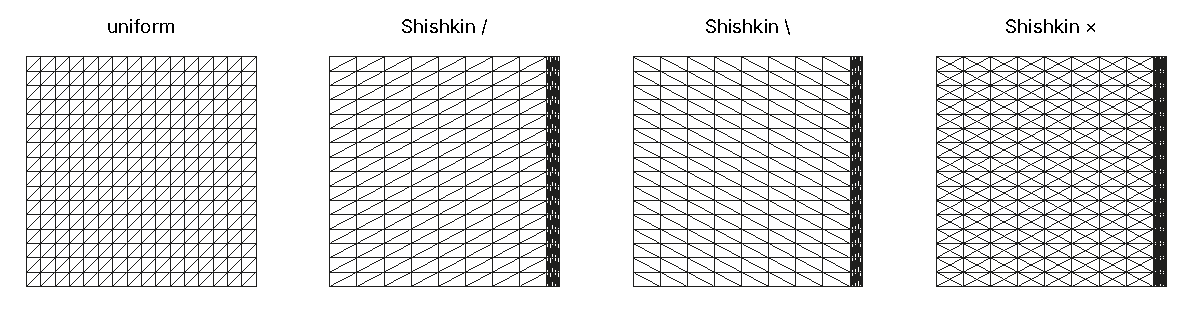
\includegraphics[width=\textwidth]{figures/aniso_meshes.pdf}
\caption{The mesh types for \texttt{parabolic\_layers}, $n=16$; drawn for $\eps=10^{-2}$ so that the layer cells are
visible (at $\eps=10^{-8}$ the layer regions have widths of order $10^{-7}$ and $10^{-3}$).}\label{fig:meshes}
\end{figure}

% generated by galerkit examples/convection_diffusion/2d/anisotropic_afc/make_report.py; do not edit
\begin{table}[!htbp]
\centering\scriptsize\setlength{\tabcolsep}{3pt}
\caption{The meshes at $n=128$: nodes, largest aspect ratio (longest edge over its height), shortest edge, largest angle, and the edges with a positive off-diagonal entry of the $P_1$ Laplace matrix (not Delaunay).}\label{tab:mesh}
\begin{tabular}{llrrrrr}
\toprule
case & mesh & nodes & aspect & $h_{\min}$ & max angle & Laplace $>0$\\
\midrule
\texttt{exp\_layer}, $\varepsilon=10^{-4}$ & uniform & 16641 & $2.0\mathrm{e}{0}$ & $7.8\mathrm{e}{-3}$ & 90.0 & 0 \\
\texttt{exp\_layer}, $\varepsilon=10^{-4}$ & Shishkin / & 16641 & $5.2\mathrm{e}{2}$ & $1.5\mathrm{e}{-5}$ & 90.0 & 0 \\
\texttt{exp\_layer}, $\varepsilon=10^{-4}$ & Shishkin \textbackslash & 16641 & $5.2\mathrm{e}{2}$ & $1.5\mathrm{e}{-5}$ & 90.0 & 0 \\
\texttt{exp\_layer}, $\varepsilon=10^{-4}$ & Shishkin $\times$ & 33025 & $1.0\mathrm{e}{3}$ & $1.5\mathrm{e}{-5}$ & 179.8 & 16320 \\
\texttt{exp\_layer}, $\varepsilon=10^{-8}$ & uniform & 16641 & $2.0\mathrm{e}{0}$ & $7.8\mathrm{e}{-3}$ & 90.0 & 0 \\
\texttt{exp\_layer}, $\varepsilon=10^{-8}$ & Shishkin / & 16641 & $5.2\mathrm{e}{6}$ & $1.5\mathrm{e}{-9}$ & 90.0 & 0 \\
\texttt{exp\_layer}, $\varepsilon=10^{-8}$ & Shishkin \textbackslash & 16641 & $5.2\mathrm{e}{6}$ & $1.5\mathrm{e}{-9}$ & 90.0 & 0 \\
\texttt{exp\_layer}, $\varepsilon=10^{-8}$ & Shishkin $\times$ & 33025 & $1.0\mathrm{e}{7}$ & $1.5\mathrm{e}{-9}$ & 180.0 & 16320 \\
\texttt{boundary\_layers}, $\varepsilon=10^{-8}$ & uniform & 16641 & $2.0\mathrm{e}{0}$ & $7.8\mathrm{e}{-3}$ & 90.0 & 0 \\
\texttt{boundary\_layers}, $\varepsilon=10^{-8}$ & Shishkin / & 16641 & $3.1\mathrm{e}{7}$ & $5.1\mathrm{e}{-10}$ & 90.0 & 0 \\
\texttt{boundary\_layers}, $\varepsilon=10^{-8}$ & Shishkin \textbackslash & 16641 & $3.1\mathrm{e}{7}$ & $5.1\mathrm{e}{-10}$ & 90.0 & 0 \\
\texttt{boundary\_layers}, $\varepsilon=10^{-8}$ & Shishkin $\times$ & 33025 & $6.2\mathrm{e}{7}$ & $4.6\mathrm{e}{-10}$ & 180.0 & 12224 \\
\texttt{parabolic\_layers}, $\varepsilon=10^{-8}$ & uniform & 16641 & $2.0\mathrm{e}{0}$ & $7.8\mathrm{e}{-3}$ & 90.0 & 0 \\
\texttt{parabolic\_layers}, $\varepsilon=10^{-8}$ & Shishkin / & 16641 & $1.0\mathrm{e}{7}$ & $1.5\mathrm{e}{-9}$ & 90.0 & 0 \\
\texttt{parabolic\_layers}, $\varepsilon=10^{-8}$ & Shishkin \textbackslash & 16641 & $1.0\mathrm{e}{7}$ & $1.5\mathrm{e}{-9}$ & 90.0 & 0 \\
\texttt{parabolic\_layers}, $\varepsilon=10^{-8}$ & Shishkin $\times$ & 33025 & $2.1\mathrm{e}{7}$ & $1.5\mathrm{e}{-9}$ & 180.0 & 16320 \\
\bottomrule
\end{tabular}
\end{table}


\paragraph{Solvers and measures.} For every algebraic method: the fixed point rhs (\texttt{fp\_rhs}), the standard
solver for these schemes, with at most 3000 iterations (efficiency); if it does not converge (Euclidean residual
$>10^{-10}$), galerkit's Newton portfolio, and for $n\le32$ in addition the Anderson-accelerated fixed point with up to
20\,000 iterations. Accuracy: the $L^2$ error, the maximal nodal error, and the maximal nodal error away from the layer
regions. The energy norm is not used: on uniform meshes the quadrature does not see layers of width $\eps$. DMP: the
mesh condition of the method checked edge by edge, the local DMP for \texttt{exp\_layer}, and the bounds of the exact
solution.

%=====================================================================================================
\section{Accuracy}
%=====================================================================================================

\begin{figure}[!htbp]\centering
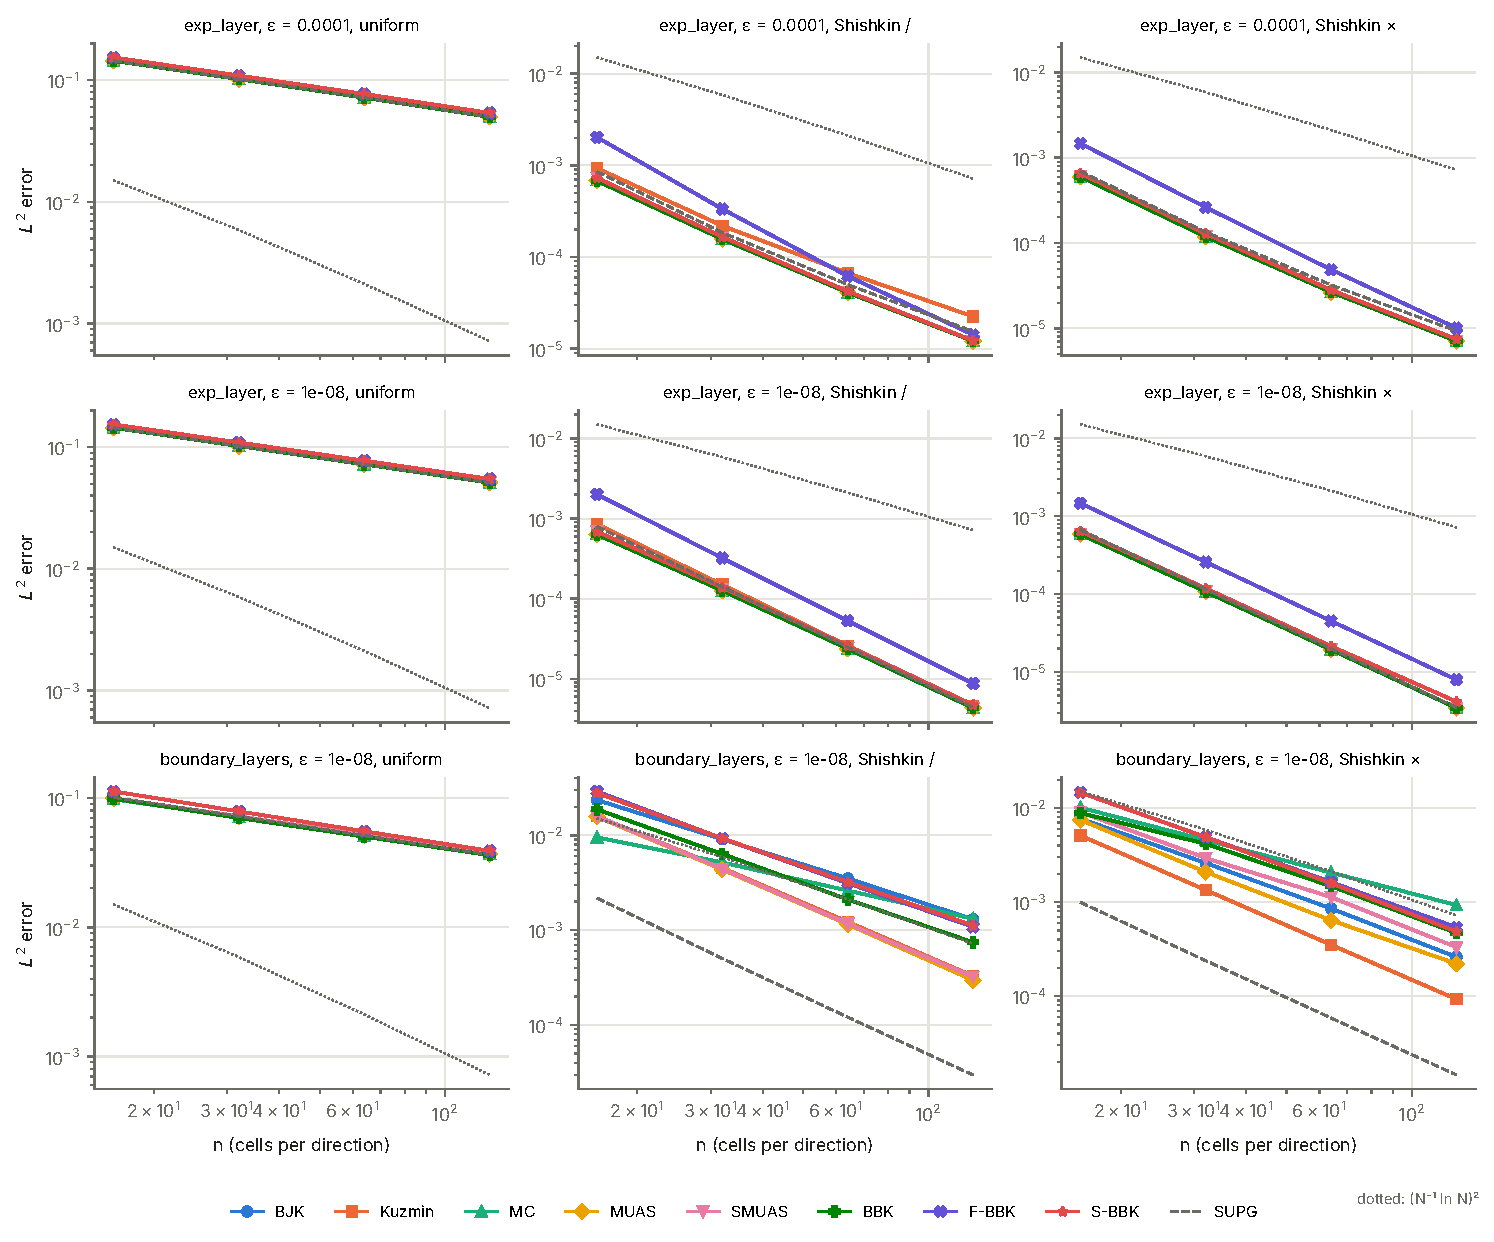
\includegraphics[width=\textwidth]{figures/aniso_errors.pdf}
\caption{$L^2$ error against $n$ on uniform, Shishkin ``/'' and crossed Shishkin meshes.}\label{fig:errors}
\end{figure}

% generated by galerkit examples/convection_diffusion/2d/anisotropic_afc/make_report.py; do not edit
\begin{table}[!htbp]
\centering\scriptsize\setlength{\tabcolsep}{3pt}
\caption{\texttt{exp\_layer}, $\varepsilon=10^{-4}$, $n=128$: maximal nodal error, its order in $n$ (between $n=64$ and 128), and the $L^2$ error.}\label{tab:acc-exp_layer-1e-04}
\begin{tabular}{l rrr rrr rrr}
\toprule
 & \multicolumn{3}{c}{uniform} & \multicolumn{3}{c}{Shishkin /} & \multicolumn{3}{c}{Shishkin $\times$}\\
method & max & ord. & $L^2$ & max & ord. & $L^2$ & max & ord. & $L^2$\\
\midrule
Galerkin & $1.6\mathrm{e}{0}$ & 0.51 & $1.6\mathrm{e}{-1}$ & $7.8\mathrm{e}{-4}$ & 1.61 & $2.3\mathrm{e}{-5}$ & $9.4\mathrm{e}{-4}$ & 1.53 & $8.1\mathrm{e}{-6}$ \\
SUPG & $2.3\mathrm{e}{-14}$ & -1.86 & $5.0\mathrm{e}{-2}$ & $1.6\mathrm{e}{-13}$ & -2.56 & $1.5\mathrm{e}{-5}$ & $8.7\mathrm{e}{-4}$ & 1.45 & $9.3\mathrm{e}{-6}$ \\
BJK & $1.6\mathrm{e}{-14}$ & -1.04 & $5.0\mathrm{e}{-2}$ & $7.7\mathrm{e}{-4}$ & 1.56 & $1.2\mathrm{e}{-5}$ & $9.4\mathrm{e}{-4}$ & 1.53 & $7.1\mathrm{e}{-6}$ \\
Kuzmin & $1.5\mathrm{e}{-14}$ & -1.01 & $5.0\mathrm{e}{-2}$ & $3.0\mathrm{e}{-3}$ & 0.95 & $2.2\mathrm{e}{-5}$ & $9.4\mathrm{e}{-4}$ & 1.53 & $7.1\mathrm{e}{-6}$ \\
MC & $1.5\mathrm{e}{-14}$ & -1.01 & $5.0\mathrm{e}{-2}$ & $7.8\mathrm{e}{-4}$ & 1.57 & $1.2\mathrm{e}{-5}$ & $9.4\mathrm{e}{-4}$ & 1.53 & $7.1\mathrm{e}{-6}$ \\
MUAS & $1.5\mathrm{e}{-14}$ & -1.01 & $5.0\mathrm{e}{-2}$ & $7.7\mathrm{e}{-4}$ & 1.56 & $1.2\mathrm{e}{-5}$ & $9.4\mathrm{e}{-4}$ & 1.53 & $7.1\mathrm{e}{-6}$ \\
SMUAS & $1.5\mathrm{e}{-14}$ & -1.01 & $5.0\mathrm{e}{-2}$ & $7.7\mathrm{e}{-4}$ & 1.56 & $1.2\mathrm{e}{-5}$ & $9.4\mathrm{e}{-4}$ & 1.53 & $7.1\mathrm{e}{-6}$ \\
BBK & $1.5\mathrm{e}{-14}$ & -1.01 & $5.0\mathrm{e}{-2}$ & $7.7\mathrm{e}{-4}$ & 1.56 & $1.2\mathrm{e}{-5}$ & $9.4\mathrm{e}{-4}$ & 1.53 & $7.1\mathrm{e}{-6}$ \\
F-BBK & $1.2\mathrm{e}{-1}$ & -0.01 & $5.4\mathrm{e}{-2}$ & $7.9\mathrm{e}{-4}$ & 1.51 & $1.4\mathrm{e}{-5}$ & $9.4\mathrm{e}{-4}$ & 1.53 & $1.0\mathrm{e}{-5}$ \\
S-BBK & $1.2\mathrm{e}{-1}$ & -0.01 & $5.4\mathrm{e}{-2}$ & $7.8\mathrm{e}{-4}$ & 1.55 & $1.2\mathrm{e}{-5}$ & $9.4\mathrm{e}{-4}$ & 1.53 & $7.4\mathrm{e}{-6}$ \\
\bottomrule
\end{tabular}
\end{table}

\begin{table}[!htbp]
\centering\scriptsize\setlength{\tabcolsep}{3pt}
\caption{\texttt{exp\_layer}, $\varepsilon=10^{-8}$, $n=128$: maximal nodal error, its order in $n$ (between $n=64$ and 128), and the $L^2$ error.}\label{tab:acc-exp_layer-1e-08}
\begin{tabular}{l rrr rrr rrr}
\toprule
 & \multicolumn{3}{c}{uniform} & \multicolumn{3}{c}{Shishkin /} & \multicolumn{3}{c}{Shishkin $\times$}\\
method & max & ord. & $L^2$ & max & ord. & $L^2$ & max & ord. & $L^2$\\
\midrule
Galerkin & $2.4\mathrm{e}{3}$ & 1.44 & $6.1\mathrm{e}{2}$ & $8.4\mathrm{e}{-4}$ & 1.59 & $7.2\mathrm{e}{-5}$ & $7.2\mathrm{e}{-3}$ & 1.15 & $4.7\mathrm{e}{-4}$ \\
SUPG & $2.8\mathrm{e}{-14}$ & -1.32 & $5.1\mathrm{e}{-2}$ & $7.2\mathrm{e}{-14}$ & -1.65 & $4.4\mathrm{e}{-6}$ & $8.7\mathrm{e}{-4}$ & 1.45 & $3.5\mathrm{e}{-6}$ \\
BJK & $1.5\mathrm{e}{-14}$ & -1.40 & $5.1\mathrm{e}{-2}$ & $7.7\mathrm{e}{-4}$ & 1.56 & $4.3\mathrm{e}{-6}$ & $9.4\mathrm{e}{-4}$ & 1.53 & $3.5\mathrm{e}{-6}$ \\
Kuzmin & $1.5\mathrm{e}{-14}$ & -1.40 & $5.1\mathrm{e}{-2}$ & $3.0\mathrm{e}{-3}$ & 0.95 & $4.5\mathrm{e}{-6}$ & $9.4\mathrm{e}{-4}$ & 1.53 & $3.5\mathrm{e}{-6}$ \\
MC & $1.5\mathrm{e}{-14}$ & -1.40 & $5.1\mathrm{e}{-2}$ & $7.8\mathrm{e}{-4}$ & 1.57 & $4.3\mathrm{e}{-6}$ & $9.4\mathrm{e}{-4}$ & 1.53 & $3.5\mathrm{e}{-6}$ \\
MUAS & $1.5\mathrm{e}{-14}$ & -1.40 & $5.1\mathrm{e}{-2}$ & $7.7\mathrm{e}{-4}$ & 1.56 & $4.3\mathrm{e}{-6}$ & $9.4\mathrm{e}{-4}$ & 1.53 & $3.5\mathrm{e}{-6}$ \\
SMUAS & $1.5\mathrm{e}{-14}$ & -1.40 & $5.1\mathrm{e}{-2}$ & $7.7\mathrm{e}{-4}$ & 1.56 & $4.3\mathrm{e}{-6}$ & $9.4\mathrm{e}{-4}$ & 1.53 & $3.5\mathrm{e}{-6}$ \\
BBK & $1.5\mathrm{e}{-14}$ & -1.40 & $5.1\mathrm{e}{-2}$ & $7.7\mathrm{e}{-4}$ & 1.56 & $4.3\mathrm{e}{-6}$ & $9.4\mathrm{e}{-4}$ & 1.53 & $3.5\mathrm{e}{-6}$ \\
F-BBK & $1.2\mathrm{e}{-1}$ & -0.00 & $5.5\mathrm{e}{-2}$ & $7.9\mathrm{e}{-4}$ & 1.51 & $8.7\mathrm{e}{-6}$ & $9.4\mathrm{e}{-4}$ & 1.53 & $8.0\mathrm{e}{-6}$ \\
S-BBK & $1.2\mathrm{e}{-1}$ & -0.00 & $5.5\mathrm{e}{-2}$ & $7.8\mathrm{e}{-4}$ & 1.55 & $4.7\mathrm{e}{-6}$ & $9.4\mathrm{e}{-4}$ & 1.53 & $4.2\mathrm{e}{-6}$ \\
\bottomrule
\end{tabular}
\end{table}

\begin{table}[!htbp]
\centering\scriptsize\setlength{\tabcolsep}{3pt}
\caption{\texttt{boundary\_layers}, $\varepsilon=10^{-8}$, $n=128$: maximal nodal error, its order in $n$ (between $n=64$ and 128), and the $L^2$ error.}\label{tab:acc-boundary_layers-1e-08}
\begin{tabular}{l rrr rrr rrr}
\toprule
 & \multicolumn{3}{c}{uniform} & \multicolumn{3}{c}{Shishkin /} & \multicolumn{3}{c}{Shishkin $\times$}\\
method & max & ord. & $L^2$ & max & ord. & $L^2$ & max & ord. & $L^2$\\
\midrule
Galerkin & $7.0\mathrm{e}{0}$ & 0.06 & $1.6\mathrm{e}{0}$ & $1.5\mathrm{e}{-2}$ & 0.78 & $6.5\mathrm{e}{-5}$ & $1.9\mathrm{e}{-3}$ & 1.34 & $3.3\mathrm{e}{-5}$ \\
SUPG & $2.9\mathrm{e}{-1}$ & -0.04 & $3.6\mathrm{e}{-2}$ & $1.7\mathrm{e}{-2}$ & 0.89 & $3.0\mathrm{e}{-5}$ & $3.2\mathrm{e}{-3}$ & 1.30 & $1.5\mathrm{e}{-5}$ \\
BJK & $5.3\mathrm{e}{-2}$ & 0.82 & $3.6\mathrm{e}{-2}$ & $2.1\mathrm{e}{-2}$ & 0.96 & $1.3\mathrm{e}{-3}$ & $1.3\mathrm{e}{-2}$ & 0.90 & $2.6\mathrm{e}{-4}$ \\
Kuzmin & $1.6\mathrm{e}{-2}$ & 0.98 & $3.7\mathrm{e}{-2}$ & $4.5\mathrm{e}{-2}$ & 0.64 & $3.3\mathrm{e}{-4}$ & $3.1\mathrm{e}{-2}$ & 0.61 & $9.3\mathrm{e}{-5}$ \\
MC & $2.5\mathrm{e}{-2}$ & 0.94 & $3.7\mathrm{e}{-2}$ & $4.0\mathrm{e}{-2}$ & 0.59 & $1.3\mathrm{e}{-3}$ & $5.9\mathrm{e}{-2}$ & 0.56 & $9.3\mathrm{e}{-4}$ \\
MUAS & $1.6\mathrm{e}{-2}$ & 0.98 & $3.7\mathrm{e}{-2}$ & $2.4\mathrm{e}{-2}$ & 0.72 & $3.0\mathrm{e}{-4}$ & $6.5\mathrm{e}{-2}$ & 0.57 & $2.2\mathrm{e}{-4}$ \\
SMUAS & $1.6\mathrm{e}{-2}$ & 0.97 & $3.7\mathrm{e}{-2}$ & $3.2\mathrm{e}{-2}$ & 0.19 & $3.2\mathrm{e}{-4}$ & $2.9\mathrm{e}{-2}$ & 1.43 & $3.3\mathrm{e}{-4}$ \\
BBK & $6.8\mathrm{e}{-2}$ & 0.74 & $3.6\mathrm{e}{-2}$ & $3.0\mathrm{e}{-2}$ & 0.67 & $7.4\mathrm{e}{-4}$ & $3.2\mathrm{e}{-2}$ & 0.56 & $4.7\mathrm{e}{-4}$ \\
F-BBK & $1.7\mathrm{e}{-1}$ & 0.21 & $3.9\mathrm{e}{-2}$ & $2.9\mathrm{e}{-2}$ & 0.97 & $1.1\mathrm{e}{-3}$ & $1.8\mathrm{e}{-2}$ & 0.97 & $5.4\mathrm{e}{-4}$ \\
S-BBK & $1.7\mathrm{e}{-1}$ & 0.21 & $3.9\mathrm{e}{-2}$ & $3.7\mathrm{e}{-2}$ & 0.69 & $1.1\mathrm{e}{-3}$ & $2.9\mathrm{e}{-2}$ & 0.69 & $4.9\mathrm{e}{-4}$ \\
\bottomrule
\end{tabular}
\end{table}


\begin{itemize}[leftmargin=*]
\item \textbf{Shishkin meshes resolve the layers} (Figure~\ref{fig:errors}). For \texttt{exp\_layer} the $L^2$ error at
  $n=128$ drops from $5\cdot10^{-2}$ on the uniform mesh to about $4\cdot10^{-6}$ ($\eps=10^{-8}$) for every method,
  with nearly the rate $(N^{-1}\ln N)^2$ and independently of $\eps$. On the uniform mesh the nodal values of this
  layer, aligned with the mesh, are exact for most methods although the layer is not resolved; the maximal nodal error
  alone is therefore not a measure of quality here.
\item \textbf{The stabilization costs accuracy where it is not needed.} For \texttt{boundary\_layers} on the
  ``/'' Shishkin mesh the Galerkin method ($L^2$ error $6.5\cdot10^{-5}$) and SUPG ($3\cdot10^{-5}$) converge with order
  2. The algebraic methods are 5--40 times less accurate: Kuzmin and MUAS $3\cdot10^{-4}$ (order about 1.9; SMUAS
  the same, but from unconverged iterates),
  BJK and BBK $0.7$--$1.3\cdot10^{-3}$ (order 1.5), MC $1.3\cdot10^{-3}$ (order 1). Away from the layers their maximal
  error, about $10^{-2}$, converges only with order 0.7--1, against 1.6--1.8 for Galerkin and SUPG. On a mesh that
  resolves the layers, the Galerkin method is stable; the artificial diffusion of the limiters then only adds a
  first-order consistency error.
\item \textbf{Splitting.} ``/'' and ``\textbackslash'' give nearly the same errors. The crossed splitting doubles the
  number of nodes and gives the same accuracy for \texttt{exp\_layer}; for \texttt{boundary\_layers} it changes the
  ordering of the methods (Kuzmin, MUAS best).
\item F-BBK is the least accurate method for \texttt{exp\_layer} (about twice the error of the others).
\end{itemize}

%=====================================================================================================
\section{Efficiency of the nonlinear solvers}
%=====================================================================================================

\begin{figure}[!htbp]\centering
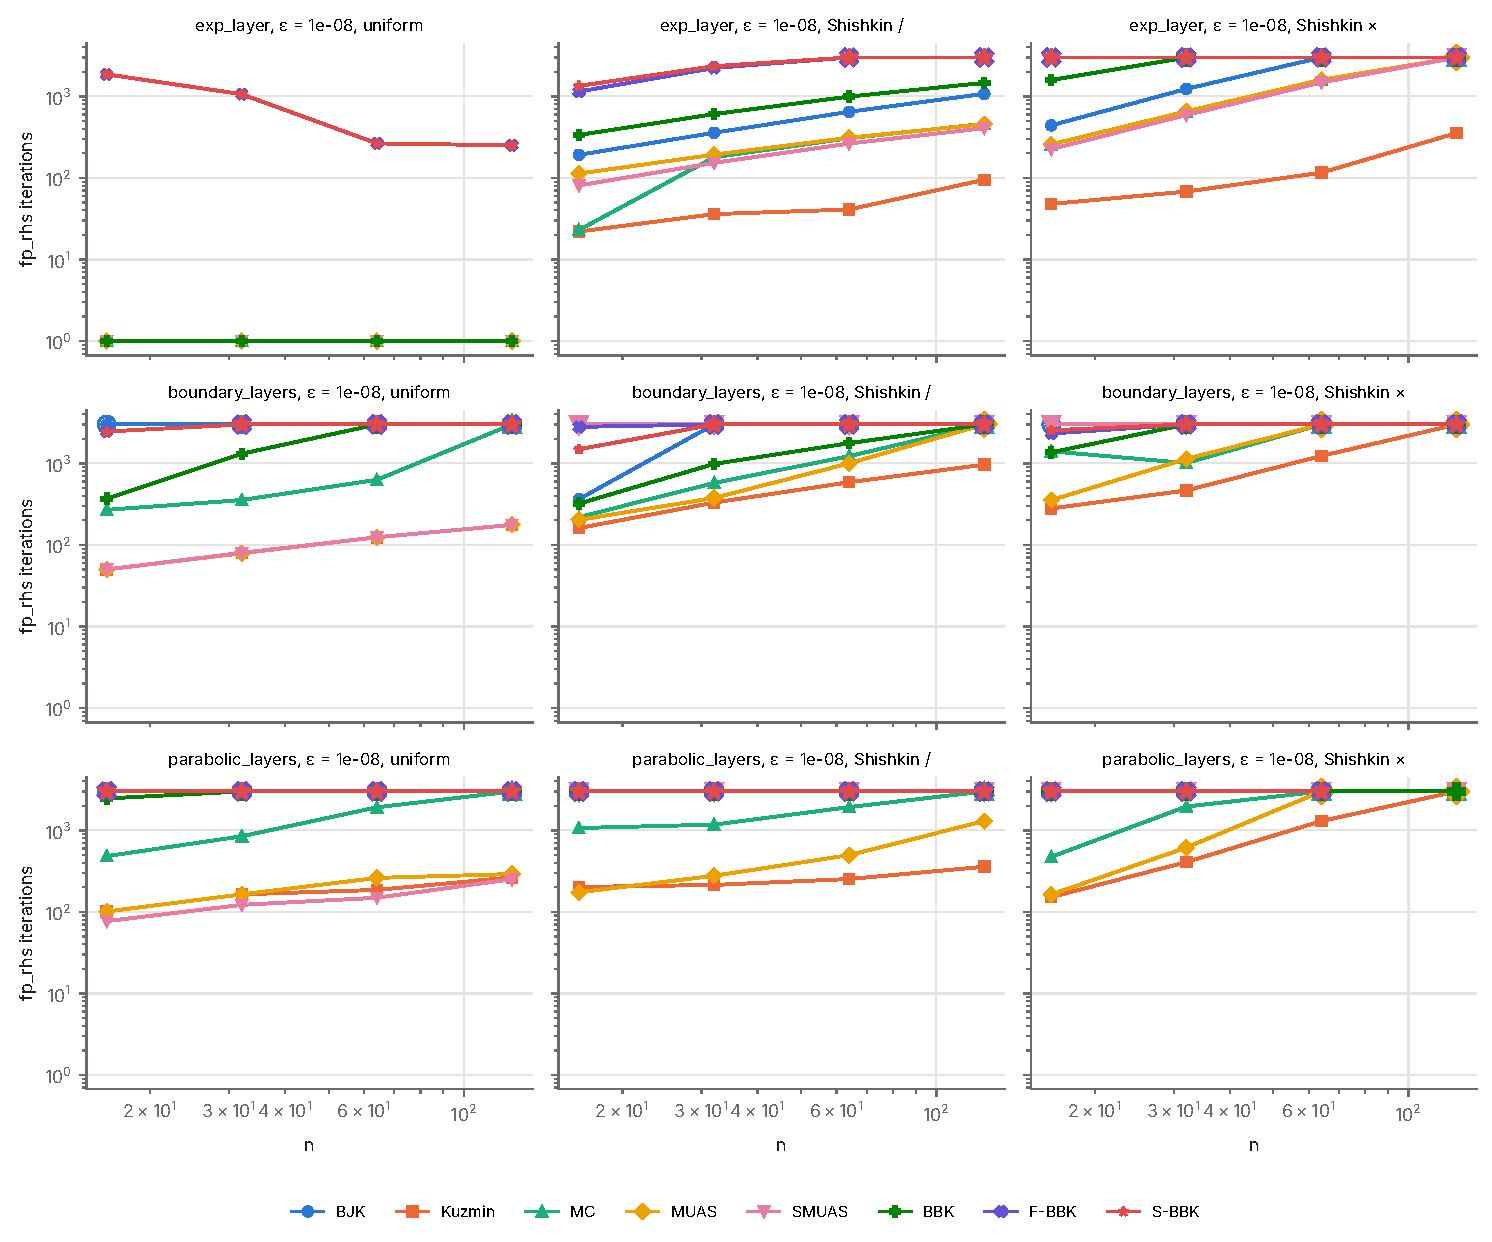
\includegraphics[width=\textwidth]{figures/aniso_iterations.pdf}
\caption{Iterations of the fixed point rhs; open circles: not converged within 3000 iterations.}\label{fig:it}
\end{figure}

% generated by galerkit examples/convection_diffusion/2d/anisotropic_afc/make_report.py; do not edit
\begin{table}[!htbp]
\centering\scriptsize\setlength{\tabcolsep}{2.5pt}
\caption{Iterations of the fixed point rhs at $n=128$ (u: uniform, /: Shishkin /, $\times$: Shishkin $\times$); in \mism{colour}: not converged within the limit (residual $>10^{-10}$).}\label{tab:eff}
\resizebox{\textwidth}{!}{\begin{tabular}{l rrr rrr rrr rrr}
\toprule
 & \multicolumn{3}{c}{\texttt{exp\_layer}, $\varepsilon=10^{-4}$} & \multicolumn{3}{c}{\texttt{exp\_layer}, $\varepsilon=10^{-8}$} & \multicolumn{3}{c}{\texttt{boundary\_layers}, $\varepsilon=10^{-8}$} & \multicolumn{3}{c}{\texttt{parabolic\_layers}, $\varepsilon=10^{-8}$}\\
method & u & / & $\times$ & u & / & $\times$ & u & / & $\times$ & u & / & $\times$\\
\midrule
BJK & 0 & 997 & \mism{3000} & 0 & 1075 & \mism{3000} & \mism{3000} & \mism{3000} & \mism{3000} & \mism{3000} & \mism{3000} & \mism{3000} \\
Kuzmin & 0 & 95 & 355 & 0 & 95 & 355 & 176 & 964 & \mism{3000} & 265 & 358 & \mism{3000} \\
MC & 0 & 454 & \mism{3000} & 0 & 461 & \mism{3000} & \mism{3000} & \mism{3000} & \mism{3000} & \mism{3000} & \mism{3000} & \mism{3000} \\
MUAS & 0 & 449 & \mism{3000} & 0 & 456 & \mism{3000} & 176 & \mism{3000} & \mism{3000} & 291 & 1298 & \mism{3000} \\
SMUAS & 0 & 406 & \mism{3000} & 0 & 408 & \mism{3000} & 176 & \mism{3000} & \mism{3000} & 252 & \mism{3000} & \mism{3000} \\
BBK & 0 & 1426 & \mism{3000} & 0 & 1465 & \mism{3000} & \mism{3000} & \mism{3000} & \mism{3000} & \mism{3000} & \mism{3000} & \mism{3000} \\
F-BBK & 246 & \mism{3000} & \mism{3000} & 251 & \mism{3000} & \mism{3000} & \mism{3000} & \mism{3000} & \mism{3000} & \mism{3000} & \mism{3000} & -- \\
S-BBK & 246 & \mism{3000} & \mism{3000} & 251 & \mism{3000} & \mism{3000} & \mism{3000} & \mism{3000} & \mism{3000} & \mism{3000} & \mism{3000} & -- \\
\bottomrule
\end{tabular}}
\end{table}


\begin{itemize}[leftmargin=*]
\item \textbf{The iteration numbers grow with the anisotropy.} Kuzmin, \texttt{exp\_layer}, $\eps=10^{-8}$, $n=128$:
  0 iterations on the uniform mesh (the low-order start is already the solution), 95 on the Shishkin ``/'' mesh, 355 on
  the crossed one. MUAS, SMUAS and MC need 400--460 iterations on the ``/'' Shishkin mesh and do not converge within 3000
  on the crossed one.
\item \textbf{Robustness of fp\_rhs} (converged runs out of 64 per method): Kuzmin 62, MUAS 56, MC 52, BBK 36, BJK 29,
  F-BBK 19, S-BBK 17. SMUAS converges on every uniform mesh but in only 22 of the 48 Shishkin runs.
\item \textbf{Not converged at all.} With the Newton portfolio and the Anderson iteration as fallbacks, 62 of the 510
  runs still end with a residual above $10^{-8}$: BJK 25, F-BBK 13, S-BBK 12 (mostly \texttt{parabolic\_layers}) and
  SMUAS 12 (all three Shishkin meshes of \texttt{boundary\_layers}). The Anderson iteration converged in none of the 28
  cases it was tried on. The errors reported for these runs are those of the best iterate.
\end{itemize}

%=====================================================================================================
\section{The DMP and the mesh conditions}
%=====================================================================================================

% generated by galerkit examples/convection_diffusion/2d/anisotropic_afc/make_report.py; do not edit
\begin{table}[!htbp]
\centering\scriptsize\setlength{\tabcolsep}{2.5pt}
\caption{DMP at $n=128$: ``ok'' if the sufficient mesh condition of the method holds on every edge, otherwise the number of edges where it fails (\mism{colour}); for \texttt{exp\_layer} ($f=c=0$) a second number gives the nodes violating the local DMP; $^\dagger$: the solution leaves the bounds of the exact solution by more than $10^{-8}$.}\label{tab:dmp}
\resizebox{\textwidth}{!}{\begin{tabular}{l rrr rrr rrr rrr}
\toprule
 & \multicolumn{3}{c}{\texttt{exp\_layer}, $\varepsilon=10^{-4}$} & \multicolumn{3}{c}{\texttt{exp\_layer}, $\varepsilon=10^{-8}$} & \multicolumn{3}{c}{\texttt{boundary\_layers}, $\varepsilon=10^{-8}$} & \multicolumn{3}{c}{\texttt{parabolic\_layers}, $\varepsilon=10^{-8}$}\\
method & u & / & $\times$ & u & / & $\times$ & u & / & $\times$ & u & / & $\times$\\
\midrule
BJK & ok & ok & ok & ok & ok & ok & ok & ok & ok & ok$^\dagger$ & ok$^\dagger$ & ok$^\dagger$ \\
Kuzmin & ok & ok & \mism{8192} & ok & ok & \mism{8192} & ok & ok & \mism{12224} & ok & ok$^\dagger$ & \mism{8192} \\
MC & ok & ok & \mism{8192} & ok & ok & \mism{8192} & ok & ok & \mism{12224} & ok & ok & \mism{8192} \\
MUAS & ok & ok & ok & ok & ok & ok & ok & ok & ok & ok & ok$^\dagger$ & ok \\
SMUAS & ok & ok & ok & ok & ok & ok & ok & ok & ok & ok & ok & ok \\
BBK & ok & ok & ok & ok & ok & ok & ok & ok & ok & ok & ok$^\dagger$ & ok \\
F-BBK & ok & ok & \mism{8064} & ok & ok & \mism{8064} & ok & ok & \mism{12224} & ok & ok$^\dagger$ & -- \\
S-BBK & ok & ok & \mism{8064} & ok & ok & \mism{8064} & ok & ok & \mism{12224} & ok & ok$^\dagger$ & -- \\
\bottomrule
\end{tabular}}
\end{table}


\begin{itemize}[leftmargin=*]
\item \textbf{Two right triangles per cell: the conditions hold.} On the uniform meshes and on the ``/'' and
  ``\textbackslash'' Shishkin meshes the Kuzmin, MC and F-/S-BBK conditions hold on every edge, for all problems. The
  diffusion matrix of right triangles has no positive off-diagonal entries, and the non-lumped reaction term of
  \texttt{boundary\_layers} ($c=1$) does not break $\min\{a_{ij},a_{ji}\}\le0$, since convection dominates.
\item \textbf{Crossed splitting: the conditions fail.} Where the layer cells are split into four triangles, the obtuse
  angles (up to $180^\circ$) make diffusion entries positive: the Kuzmin/MC condition fails on 128 to 12\,224 edges,
  the F-/S-BBK condition at the larger $n$ (8\,064 edges for \texttt{exp\_layer} at $n=128$).
\item \textbf{No observed DMP violation.} For \texttt{exp\_layer}, where the local DMP applies, no method violates it on
  any mesh, including Kuzmin and MC on the crossed meshes where their condition fails. For
  \texttt{parabolic\_layers} no method undershoots $u\ge0$.
\item \textbf{Overshoots of the exact bound.} On the ``/'' and ``\textbackslash'' Shishkin meshes of
  \texttt{parabolic\_layers}, BJK, Kuzmin, MUAS, BBK, F-BBK and S-BBK exceed the bound $u\le1$ of the exact solution by
  up to 2--9\,\%; this is not a DMP violation ($f=1$), but non-physical. MC and SMUAS stay below $1+6\cdot10^{-4}$, and
  no method overshoots on the crossed meshes.
\end{itemize}

%=====================================================================================================
\section{Switching the stabilization off where the mesh resolves the layer}\label{sec:roff}
%=====================================================================================================

\paragraph{The switch.} With the flag \texttt{afc\_resolved\_off=True} of \texttt{CDRSolver} (default \texttt{False}),
every edge $E=\overline{x_ix_j}$ with mesh P\'eclet number
\[
  \mathrm{Pe}_E=\frac{|\bb(x_E)|\,|x_j-x_i|}{2\eps(x_E)}\le\mathrm{Pe}^*\qquad(\mathrm{Pe}^*=1,\ \texttt{afc\_pe\_threshold})
\]
gets $d_{ij}=b_{ij}=0$: the scheme is the Galerkin method on the edges where the mesh resolves the solution. It acts on
all eight methods through an edge mask of \texttt{AFCOperator}. The full speed $|\bb|$ is used: with its component
along the edge, $|\bb\cdot(x_j-x_i)|$, every edge orthogonal to the flow would count as resolved, and the crosswind
edges of the coarse cells (e.g.\ all vertical edges for $\bb=(1,0)$) would be switched off everywhere.

\paragraph{Already switched off there.} The artificial diffusion of the algebraic methods,
\[
  d_{ij}=-\max\{a_{ij},0,a_{ji}\},
\]
vanishes on every edge with $\max\{a_{ij},a_{ji}\}\le0$, which is the case on a diffusion-dominated edge of a right
triangle. At $n=128$ the meshes have between 8\,128 and 32\,640 edges
with $\mathrm{Pe}_E\le1$. For the problems \texttt{exp\_layer} and \texttt{parabolic\_layers}, none of them has
$d_{ij}\ne0$, so the switch changes nothing there. For
\texttt{boundary\_layers} it acts on about 4\,000 edges at $n=128$ where the reaction term ($c=1$, not lumped) makes
$\max\{a_{ij},a_{ji}\}>0$; switching them off loses the DMP guarantee on exactly these edges.

% generated by galerkit examples/convection_diffusion/2d/anisotropic_afc/make_report.py; do not edit
\begin{table}[!htbp]
\centering\scriptsize\setlength{\tabcolsep}{2.5pt}
\caption{\texttt{boundary\_layers}, $\varepsilon=10^{-8}$: $L^2$ error and fixed point rhs iterations with the stabilization everywhere / switched off on the edges with $|\bb||E|/(2\varepsilon)\le1$ (\texttt{afc\_resolved\_off}); $^*$: final residual $>10^{-8}$. Galerkin on the Shishkin ``/'' mesh, $n=128$: $6.5\mathrm{e}{-5}$.}\label{tab:roff}
\resizebox{\textwidth}{!}{\begin{tabular}{l rr rr rr rr}
\toprule
 & \multicolumn{4}{c}{Shishkin /} & \multicolumn{4}{c}{Shishkin $\times$}\\
 & \multicolumn{2}{c}{$n=64$} & \multicolumn{2}{c}{$n=128$} & \multicolumn{2}{c}{$n=64$} & \multicolumn{2}{c}{$n=128$}\\
method & $L^2$ & it. & $L^2$ & it. & $L^2$ & it. & $L^2$ & it.\\
\midrule
BJK & $3.5\mathrm{e}{-3}$ / $3.5\mathrm{e}{-3}$ & 3000 / 3000 & $1.3\mathrm{e}{-3}$$^*$ / $1.3\mathrm{e}{-3}$$^*$ & 3000 / 3000 & $8.5\mathrm{e}{-4}$$^*$ / $8.5\mathrm{e}{-4}$$^*$ & 3000 / 3000 & $2.6\mathrm{e}{-4}$$^*$ / $3.0\mathrm{e}{-4}$$^*$ & 3000 / 3000 \\
Kuzmin & $1.2\mathrm{e}{-3}$ / $1.2\mathrm{e}{-3}$ & 587 / 587 & $3.3\mathrm{e}{-4}$ / $3.3\mathrm{e}{-4}$ & 964 / 964 & $3.5\mathrm{e}{-4}$ / $3.5\mathrm{e}{-4}$ & 1233 / 1233 & $9.3\mathrm{e}{-5}$ / $9.3\mathrm{e}{-5}$ & 3000 / 3000 \\
MC & $2.6\mathrm{e}{-3}$ / $2.6\mathrm{e}{-3}$ & 1225 / 1225 & $1.3\mathrm{e}{-3}$ / $1.3\mathrm{e}{-3}$ & 3000 / 3000 & $2.1\mathrm{e}{-3}$ / $2.1\mathrm{e}{-3}$ & 3000 / 3000 & $9.3\mathrm{e}{-4}$ / $9.3\mathrm{e}{-4}$ & 3000 / 3000 \\
MUAS & $1.2\mathrm{e}{-3}$ / $1.2\mathrm{e}{-3}$ & 1001 / 1001 & $3.0\mathrm{e}{-4}$ / $3.0\mathrm{e}{-4}$ & 3000 / 3000 & $6.4\mathrm{e}{-4}$ / $6.4\mathrm{e}{-4}$ & 3000 / 3000 & $2.2\mathrm{e}{-4}$ / $2.2\mathrm{e}{-4}$ & 3000 / 3000 \\
SMUAS & $1.2\mathrm{e}{-3}$$^*$ / $1.2\mathrm{e}{-3}$$^*$ & 3000 / 3000 & $3.2\mathrm{e}{-4}$$^*$ / $3.2\mathrm{e}{-4}$$^*$ & 3000 / 3000 & $1.1\mathrm{e}{-3}$$^*$ / $1.1\mathrm{e}{-3}$$^*$ & 3000 / 3000 & $3.3\mathrm{e}{-4}$$^*$ / $4.0\mathrm{e}{-4}$$^*$ & 3000 / 3000 \\
BBK & $2.1\mathrm{e}{-3}$ / $2.1\mathrm{e}{-3}$ & 1768 / 1767 & $7.4\mathrm{e}{-4}$ / $7.4\mathrm{e}{-4}$ & 3000 / 3000 & $1.5\mathrm{e}{-3}$ / $1.5\mathrm{e}{-3}$$^*$ & 3000 / 3000 & $4.7\mathrm{e}{-4}$ / $4.7\mathrm{e}{-4}$$^*$ & 3000 / 3000 \\
F-BBK & $3.1\mathrm{e}{-3}$ / $3.1\mathrm{e}{-3}$ & 3000 / 3000 & $1.1\mathrm{e}{-3}$ / $1.1\mathrm{e}{-3}$ & 3000 / 3000 & $1.6\mathrm{e}{-3}$ / $1.6\mathrm{e}{-3}$ & 3000 / 3000 & $5.4\mathrm{e}{-4}$ / $5.4\mathrm{e}{-4}$ & 3000 / 3000 \\
S-BBK & $3.2\mathrm{e}{-3}$ / $3.2\mathrm{e}{-3}$ & 3000 / 3000 & $1.1\mathrm{e}{-3}$ / $1.1\mathrm{e}{-3}$ & 3000 / 3000 & $1.6\mathrm{e}{-3}$ / $1.6\mathrm{e}{-3}$$^*$ & 3000 / 3000 & -- & -- \\
\bottomrule
\end{tabular}}
\end{table}


\paragraph{Result: it does not help} (Table~\ref{tab:roff}). For \texttt{boundary\_layers} the $L^2$ errors and the
iteration numbers are unchanged within a few per cent (Kuzmin, Shishkin ``/'', $n=128$: $3.3\cdot10^{-4}$ in both
cases, Galerkin $6.5\cdot10^{-5}$); BJK and SMUAS on the crossed mesh become slightly worse. The reason is where the
error comes from: in the interior of the coarse region the algebraic methods are as accurate as the Galerkin method
($1.9\cdot10^{-3}$ against $1.5\cdot10^{-3}$ at $n=64$); their large error ($2.3\cdot10^{-2}$) sits at the transition
corner $(1-\tau_x,1-\tau_y)$. It is caused by the long edges inside the layer strips (length $1/n$ along the layer,
$\mathrm{Pe}_E\gg1$ since $\bb=(2,3)$ has a component along them): there the limiters add diffusion along the layer,
the P\'eclet criterion correctly regards these edges as unresolved, and the switch does not touch them. Reducing this
error needs a criterion that sees the resolution of the solution, not only of the mesh (e.g.\ the limiter switched
off on edges inside the layer region along the layer).

%=====================================================================================================
\section{Switching the limiter off along the layers}\label{sec:loff}
%=====================================================================================================

\paragraph{The switch.} With \texttt{afc\_layer\_off=True} (default \texttt{False}), $d_{ij}=b_{ij}=0$ on the edges
that run along a layer: edges whose adjacent cells all have aspect ratio
$\mathrm{diam}(K)^2/(2|K|)$ at least 10 (the option \texttt{afc\_aspect\_threshold}), and on which the edge is a long edge
($|E|\ge\frac12\mathrm{diam}(K)$) of every adjacent cell. These are exactly the edges named at the end of
Section~\ref{sec:roff}. The switch knows only the mesh; on a layer-adapted mesh the long edges inside the layer strips
are where the solution varies slowly. \texttt{dmp\_certificate} counts the switched-off edges with
$\max\{a_{ij},a_{ji}\}>0$, where the DMP guarantee is lost.

\paragraph{Iterations.} Median fixed point rhs iterations over the 16 runs per mesh and method (four cases, $n=16$ to
$128$), counted over the runs that converge with and without the switch, Shishkin ``/'' mesh: BJK $490\to10$, Kuzmin
$128\to26$, MC $381\to15$, MUAS $308\to17$, SMUAS $209\to7$, BBK $983\to35$, S-BBK $2300\to200$; the number of
converged runs does not decrease, except BJK ($9\to8$) and F-BBK ($5\to4$). On the crossed mesh the converged runs
increase (BJK $4\to8$, MUAS $10\to14$, SMUAS $6\to12$, F-/S-BBK $1\to9$), except for BBK. Table~\ref{tab:lm-it} gives
the numbers at $n=128$: for \texttt{exp\_layer} 5--10 iterations instead of 95--1465, for \texttt{boundary\_layers}
Kuzmin and MUAS need 128 instead of 964 and $>3000$.

\paragraph{Accuracy.} For \texttt{exp\_layer} the errors are unchanged on the Shishkin mesh. For
\texttt{boundary\_layers} the error at the transition corner drops: Kuzmin, $n=128$, maximal error away from the layers
$1.4\cdot10^{-2}\to2.5\cdot10^{-3}$, MUAS $6.9\cdot10^{-3}\to2.7\cdot10^{-3}$, with the $L^2$ error $3.3\to2.9\cdot10^{-4}$
(Table~\ref{tab:lm-acc}). For \texttt{parabolic\_layers} the overshoot of Kuzmin and MUAS grows slightly
($\max u_h=1.008\to1.013$ at $n=128$), while MC no longer stays below 1 but reaches $1+3\cdot10^{-4}$. No local DMP
violation occurs for \texttt{exp\_layer}.

%=====================================================================================================
\section{Other layer-adapted meshes and the number of iterations}\label{sec:meshes}
%=====================================================================================================

\paragraph{Question.} Shishkin meshes are piecewise uniform: at the transition point the step size jumps from
$O(\eps\ln N/N)$ to $O(1/N)$. Do meshes with a smoother transition need fewer nonlinear iterations? We compare, with
the same number of cells in the layer region ($n/2$ per direction, $\sigma=2$, ``/'' diagonals;
\texttt{galerkit.core.mesh.layer\_points}):
\begin{itemize}[leftmargin=*]
\item \textbf{Bakhvalov--Shishkin} (Linß): $x_i=-\sigma\eps/\beta\,\ln\bigl(1-(1-N^{-1})\,i/(qN)\bigr)$ in the layer
  region, $q=\frac12$, uniform outside; the step size grows smoothly up to the transition point;
\item \textbf{Bakhvalov}: the mesh generating function $\varphi(t)=-\sigma\eps/\beta\,\ln(1-t/q)$ continued by its
  tangent through $(1,1)$, a $C^1$ mesh generating function;
\item \textbf{Dur\'an--Lombardi}: $x_i=ih\eps$ up to $\eps$, then $x_{i+1}=(1+h)x_i$, $h$ chosen for $N$ cells; geometric
  grading with ratio $1+h$ and no transition point.
\end{itemize}
All three are anisotropic in the layer region as the Shishkin mesh; 480 runs, Tables~\ref{tab:lm-it}
and~\ref{tab:lm-acc}.

% generated by galerkit examples/convection_diffusion/2d/anisotropic_afc/make_report.py; do not edit
\begin{table}[!htbp]
\centering\scriptsize\setlength{\tabcolsep}{3pt}
\caption{Iterations of the fixed point rhs at $n=128$ on the layer-adapted meshes (``/'' diagonals); ``+ off'': limiter switched off along the layers (\texttt{afc\_layer\_off}); in \mism{colour}: not converged within 3000 iterations.}\label{tab:lm-it}
\begin{tabular}{l rrrrrrrr}
\toprule
mesh & BJK & Kuzmin & MC & MUAS & SMUAS & BBK & F-BBK & S-BBK\\
\midrule
\multicolumn{9}{l}{\texttt{exp\_layer}, $\varepsilon=10^{-4}$}\\
uniform & 0 & 0 & 0 & 0 & 0 & 0 & 246 & 246 \\
Shishkin & 997 & 95 & 454 & 449 & 406 & 1426 & \mism{3000} & \mism{3000} \\
Bakhvalov--Shishkin & \mism{3000} & 143 & 226 & 236 & 241 & 736 & \mism{3000} & \mism{3000} \\
Bakhvalov & \mism{3000} & 143 & 233 & 231 & 262 & 689 & \mism{3000} & 2772 \\
Dur\'an--Lombardi & 2693 & 55 & 214 & 253 & 250 & 255 & \mism{3000} & \mism{3000} \\
Shishkin + off & 6 & 7 & 6 & 9 & 6 & 5 & \mism{3000} & \mism{3000} \\
Bakhvalov--Shishkin + off & 440 & 9 & 9 & 9 & 9 & 7 & \mism{3000} & \mism{3000} \\
Bakhvalov + off & 145 & 9 & 9 & 8 & 6 & 26 & \mism{3000} & 161 \\
\midrule
\multicolumn{9}{l}{\texttt{exp\_layer}, $\varepsilon=10^{-8}$}\\
uniform & 0 & 0 & 0 & 0 & 0 & 0 & 251 & 251 \\
Shishkin & 1075 & 95 & 461 & 456 & 408 & 1465 & \mism{3000} & \mism{3000} \\
Bakhvalov--Shishkin & \mism{3000} & 143 & 227 & 238 & 241 & 748 & \mism{3000} & \mism{3000} \\
Bakhvalov & \mism{3000} & 143 & 234 & 230 & 268 & 750 & \mism{3000} & 2992 \\
Dur\'an--Lombardi & \mism{3000} & 29 & 102 & 148 & 140 & 221 & \mism{3000} & \mism{3000} \\
Shishkin + off & 7 & 7 & 7 & 10 & 6 & 6 & \mism{3000} & \mism{3000} \\
Bakhvalov--Shishkin + off & 50 & 8 & 10 & 8 & 8 & 7 & 344 & 176 \\
Bakhvalov + off & \mism{3000} & 6 & 8 & 6 & 6 & 34 & 297 & 301 \\
\midrule
\multicolumn{9}{l}{\texttt{boundary\_layers}, $\varepsilon=10^{-8}$}\\
uniform & \mism{3000} & 176 & \mism{3000} & 176 & 176 & \mism{3000} & \mism{3000} & \mism{3000} \\
Shishkin & \mism{3000} & 964 & \mism{3000} & \mism{3000} & \mism{3000} & \mism{3000} & \mism{3000} & \mism{3000} \\
Bakhvalov--Shishkin & \mism{3000} & 462 & 1623 & 643 & \mism{3000} & 2241 & \mism{3000} & \mism{3000} \\
Bakhvalov & \mism{3000} & 413 & 1537 & 592 & \mism{3000} & 2275 & \mism{3000} & \mism{3000} \\
Dur\'an--Lombardi & 618 & 669 & 1313 & 654 & 200 & 685 & 2972 & 2981 \\
Shishkin + off & \mism{3000} & 128 & 1522 & 128 & \mism{3000} & 2228 & \mism{3000} & \mism{3000} \\
Bakhvalov--Shishkin + off & \mism{3000} & 128 & 1609 & 128 & \mism{3000} & 2230 & \mism{3000} & \mism{3000} \\
Bakhvalov + off & \mism{3000} & 128 & 1612 & 128 & \mism{3000} & 2253 & \mism{3000} & \mism{3000} \\
\midrule
\multicolumn{9}{l}{\texttt{parabolic\_layers}, $\varepsilon=10^{-8}$}\\
uniform & \mism{3000} & 265 & \mism{3000} & 291 & 252 & \mism{3000} & \mism{3000} & \mism{3000} \\
Shishkin & \mism{3000} & 358 & \mism{3000} & 1298 & \mism{3000} & \mism{3000} & \mism{3000} & \mism{3000} \\
Bakhvalov--Shishkin & \mism{3000} & 325 & \mism{3000} & 524 & \mism{3000} & \mism{3000} & \mism{3000} & \mism{3000} \\
Bakhvalov & \mism{3000} & 363 & \mism{3000} & 508 & \mism{3000} & \mism{3000} & \mism{3000} & \mism{3000} \\
Dur\'an--Lombardi & \mism{3000} & 1175 & 1006 & 1181 & 297 & 1407 & \mism{3000} & \mism{3000} \\
Shishkin + off & \mism{3000} & 342 & 2335 & 343 & \mism{3000} & \mism{3000} & \mism{3000} & \mism{3000} \\
Bakhvalov--Shishkin + off & \mism{3000} & 312 & 2261 & 316 & \mism{3000} & \mism{3000} & \mism{3000} & \mism{3000} \\
Bakhvalov + off & \mism{3000} & 254 & 2654 & 328 & \mism{3000} & \mism{3000} & \mism{3000} & \mism{3000} \\
\bottomrule
\end{tabular}
\end{table}

% generated by galerkit examples/convection_diffusion/2d/anisotropic_afc/make_report.py; do not edit
\begin{table}[!htbp]
\centering\scriptsize\setlength{\tabcolsep}{2.5pt}
\caption{Accuracy on the layer-adapted meshes, $n=128$, $\varepsilon=10^{-8}$: $L^2$ error and maximal nodal error away from the layers for Galerkin, Kuzmin and MUAS; last column: $\max u_h$ of Kuzmin for \texttt{parabolic\_layers} (exact bound 1).}\label{tab:lm-acc}
\resizebox{\textwidth}{!}{\begin{tabular}{l rrrrrr rrrrrr r}
\toprule
 & \multicolumn{6}{c}{\texttt{exp\_layer}} & \multicolumn{6}{c}{\texttt{boundary\_layers}} & parab.\\
 & \multicolumn{2}{c}{Galerkin} & \multicolumn{2}{c}{Kuzmin} & \multicolumn{2}{c}{MUAS} & \multicolumn{2}{c}{Galerkin} & \multicolumn{2}{c}{Kuzmin} & \multicolumn{2}{c}{MUAS} & Kuzmin\\
mesh & $L^2$ & away & $L^2$ & away & $L^2$ & away & $L^2$ & away & $L^2$ & away & $L^2$ & away & $\max u_h$\\
\midrule
uniform & $6.1\mathrm{e}{2}$ & $2.4\mathrm{e}{3}$ & $5.1\mathrm{e}{-2}$ & $1.5\mathrm{e}{-14}$ & $5.1\mathrm{e}{-2}$ & $1.5\mathrm{e}{-14}$ & $1.6\mathrm{e}{0}$ & $7.0\mathrm{e}{0}$ & $3.7\mathrm{e}{-2}$ & $1.6\mathrm{e}{-2}$ & $3.7\mathrm{e}{-2}$ & $1.6\mathrm{e}{-2}$ & 0.998 \\
Shishkin & $7.2\mathrm{e}{-5}$ & $2.6\mathrm{e}{-4}$ & $4.5\mathrm{e}{-6}$ & $1.1\mathrm{e}{-5}$ & $4.3\mathrm{e}{-6}$ & $9.3\mathrm{e}{-6}$ & $6.5\mathrm{e}{-5}$ & $4.8\mathrm{e}{-4}$ & $3.3\mathrm{e}{-4}$ & $1.4\mathrm{e}{-2}$ & $3.0\mathrm{e}{-4}$ & $6.9\mathrm{e}{-3}$ & 1.008 \\
Bakhvalov--Shishkin & $2.5\mathrm{e}{-5}$ & $1.1\mathrm{e}{-4}$ & $3.0\mathrm{e}{-6}$ & $2.0\mathrm{e}{-5}$ & $2.6\mathrm{e}{-6}$ & $2.6\mathrm{e}{-5}$ & $8.5\mathrm{e}{-5}$ & $6.6\mathrm{e}{-4}$ & $2.9\mathrm{e}{-4}$ & $4.4\mathrm{e}{-3}$ & $2.9\mathrm{e}{-4}$ & $3.2\mathrm{e}{-3}$ & 1.013 \\
Bakhvalov & $1.7\mathrm{e}{-4}$ & $6.2\mathrm{e}{-4}$ & $6.6\mathrm{e}{-8}$ & $6.2\mathrm{e}{-15}$ & $5.3\mathrm{e}{-8}$ & $6.0\mathrm{e}{-15}$ & $1.5\mathrm{e}{-4}$ & $1.2\mathrm{e}{-3}$ & $3.0\mathrm{e}{-4}$ & $4.9\mathrm{e}{-3}$ & $2.9\mathrm{e}{-4}$ & $3.3\mathrm{e}{-3}$ & 1.015 \\
Dur\'an--Lombardi & $1.5\mathrm{e}{-7}$ & $4.2\mathrm{e}{-5}$ & $3.1\mathrm{e}{-7}$ & $7.4\mathrm{e}{-6}$ & $1.5\mathrm{e}{-7}$ & $1.3\mathrm{e}{-5}$ & $4.0\mathrm{e}{-3}$ & $6.3\mathrm{e}{-3}$ & $5.7\mathrm{e}{-3}$ & $3.5\mathrm{e}{-2}$ & $5.7\mathrm{e}{-3}$ & $3.5\mathrm{e}{-2}$ & 1.000 \\
Shishkin + off & -- & -- & $4.3\mathrm{e}{-6}$ & $7.4\mathrm{e}{-6}$ & $4.3\mathrm{e}{-6}$ & $9.3\mathrm{e}{-6}$ & -- & -- & $2.9\mathrm{e}{-4}$ & $2.5\mathrm{e}{-3}$ & $2.9\mathrm{e}{-4}$ & $2.7\mathrm{e}{-3}$ & 1.013 \\
Bakhvalov--Shishkin + off & -- & -- & $1.5\mathrm{e}{-6}$ & $9.2\mathrm{e}{-5}$ & $1.5\mathrm{e}{-6}$ & $9.2\mathrm{e}{-5}$ & -- & -- & $2.9\mathrm{e}{-4}$ & $2.3\mathrm{e}{-3}$ & $2.9\mathrm{e}{-4}$ & $2.5\mathrm{e}{-3}$ & 1.012 \\
Bakhvalov + off & -- & -- & $2.3\mathrm{e}{-6}$ & $4.1\mathrm{e}{-5}$ & $2.3\mathrm{e}{-6}$ & $4.1\mathrm{e}{-5}$ & -- & -- & $2.9\mathrm{e}{-4}$ & $2.2\mathrm{e}{-3}$ & $2.9\mathrm{e}{-4}$ & $2.4\mathrm{e}{-3}$ & 1.011 \\
\bottomrule
\end{tabular}}
\end{table}


\paragraph{Results without the switch.}
\begin{itemize}[leftmargin=*]
\item \textbf{Bakhvalov--Shishkin and Bakhvalov} reduce by about half the iterations of MC, MUAS and BBK for
  \texttt{exp\_layer} and of
  Kuzmin, MC and MUAS for \texttt{boundary\_layers} (at $n=128$: Kuzmin $964\to413$, MUAS $>3000\to592$), and they
  are slightly more accurate there. Kuzmin on \texttt{exp\_layer} needs more iterations ($95\to143$), BJK no longer
  converges at all (0--1 of 16 runs, against 9 of 16), and SMUAS and F-/S-BBK remain unreliable. On the Bakhvalov mesh the
  algebraic methods are nodally exact away from the layer for \texttt{exp\_layer} ($L^2$ error $6.6\cdot10^{-8}$).
\item \textbf{Dur\'an--Lombardi} gives the fewest iterations for \texttt{exp\_layer} (Kuzmin 29 at $n=128$) and lets SMUAS
  and BJK converge for \texttt{boundary\_layers}. But at these $N$ the grading $1+h$ is large and its coarsest cells are
  much larger than $1/N$: for \texttt{boundary\_layers} the $L^2$ error is 20 times larger than on the other meshes
  ($5.7\cdot10^{-3}$ for Kuzmin at $n=128$), and for \texttt{parabolic\_layers} Kuzmin and MUAS need three times more
  iterations (1175 against 358). It does not suit layers in two directions at moderate $N$.
\end{itemize}

\paragraph{Results with the switch.} With \texttt{afc\_layer\_off} the mesh type hardly matters any more for Kuzmin,
MC and MUAS: at $n=128$, 6--10 iterations for \texttt{exp\_layer}, 128 for \texttt{boundary\_layers}, 250--340 for
\texttt{parabolic\_layers}, on all three meshes. The switch cuts the iterations by a factor 3--50, the choice of mesh by
at most a factor 2. On the Bakhvalov meshes the switch costs accuracy for \texttt{exp\_layer} ($L^2$ error
$6.6\cdot10^{-8}\to2.3\cdot10^{-6}$), since it replaces the nodally exact limiter by the Galerkin method on the graded
cells; on the Shishkin mesh it costs nothing.

\paragraph{The best choice for few iterations.} \emph{The Shishkin mesh with the limiter switched off along the layers,
with Kuzmin or MUAS}: the fewest iterations in all four cases, the smallest errors away from the layers for
\texttt{boundary\_layers}, and the simplest mesh. Bakhvalov--Shishkin with the switch is as good (and gives F-/S-BBK a
chance), Bakhvalov without it is the best mesh for an aligned exponential layer.

\paragraph{What the mesh cannot fix.} BJK, SMUAS, BBK, F-BBK and S-BBK fail for \texttt{boundary\_layers} and
\texttt{parabolic\_layers} also on uniform meshes (Table~\ref{tab:eff}); their failures are a property of the limiter
and the fixed point iteration, not of the anisotropy. For these the sharper tools are on the solver side: damped and
Anderson-accelerated fixed point iterations and Newton methods (compared for AFC by Jha and John), or differentiable
(regularized) limiters that make Newton's method applicable (Badia and Bonilla). The switch along the layers remains
useful with any of them, since it removes the nonlinearity from the edges where it is not needed.

%=====================================================================================================
\section{Anderson acceleration with the switch}\label{sec:aa}
%=====================================================================================================

\paragraph{Solvers.} The fixed point rhs, $(A+D)\tilde u=g-L(\boldsymbol b(u^k)-\boldsymbol d)u^k$, uses one
factorization and a residual-based damping $u^{k+1}=u^k+\omega(\tilde u-u^k)$. Its Anderson acceleration
(\texttt{fp\_anderson}, depth 10, Walker--Ni) combines the last 10 fixed point images by least squares, without damping,
and restarts from the best iterate if the residual has not halved within 200 iterations. For F-BBK and S-BBK the
undamped fixed point map is expansive (residual $1.6\to2.4\cdot10^1\to\dots\to10^{14}$ in 30 iterations on a uniform
$16\times16$ mesh), and Anderson diverges. The new variant \texttt{fp\_anderson\_safe} accepts an accelerated iterate
only if its residual is below the largest of the last 10 residuals (non-monotone, since Anderson is not monotone);
otherwise it takes the damped fixed point step and clears the history. A monotone test (window 1) rejects about every
second step and destroys the acceleration (BJK and BBK no longer converge); windows 5--30 were tested, 10 is the
best compromise. Runs: all eight algebraic methods, four cases, $n=16$--$128$, on the uniform mesh, the Shishkin
``/'' mesh without and with \texttt{afc\_layer\_off}, and the crossed Shishkin mesh with it (512 runs per solver;
the safeguarded variant misses the 33 runs of \texttt{parabolic\_layers} at $n=128$, stopped). Table~\ref{tab:aa}.

% generated by galerkit examples/convection_diffusion/2d/anisotropic_afc/make_report.py; do not edit
\begin{table}[!htbp]
\centering\scriptsize\setlength{\tabcolsep}{3pt}
\caption{Iterations at $n=128$: fixed point rhs and its Anderson acceleration (depth 10, restart after 200 iterations without halving the residual; safeg.: with the non-monotone residual safeguard, window 10), without and with the limiter switched off along the layers (``+ off''); in \mism{colour}: not converged within 3000 iterations; \texttt{exp\_layer} with $\varepsilon=10^{-4}$ gives the same picture.}\label{tab:aa}
\resizebox{\textwidth}{!}{\begin{tabular}{l rrrrrrrr}
\toprule
mesh, solver & BJK & Kuzmin & MC & MUAS & SMUAS & BBK & F-BBK & S-BBK\\
\midrule
\multicolumn{9}{l}{\texttt{exp\_layer}, $\varepsilon=10^{-8}$}\\
uniform, fp rhs & 0 & 0 & 0 & 0 & 0 & 0 & 251 & 251 \\
uniform, Anderson & 0 & 0 & 0 & 0 & 0 & 0 & \mism{3000} & \mism{3000} \\
uniform, Anderson, safeg. & 0 & 0 & 0 & 0 & 0 & 0 & 275 & 275 \\
Shishkin /, fp rhs & 1075 & 95 & 461 & 456 & 408 & 1465 & \mism{3000} & \mism{3000} \\
Shishkin /, Anderson & 273 & 37 & 55 & 47 & 44 & 434 & \mism{3000} & \mism{3000} \\
Shishkin /, Anderson, safeg. & 280 & 37 & 55 & 47 & 44 & 976 & 2578 & 2521 \\
Shishkin / + off, fp rhs & 7 & 7 & 7 & 10 & 6 & 6 & \mism{3000} & \mism{3000} \\
Shishkin / + off, Anderson & 4 & 5 & 4 & 5 & 4 & 6 & \mism{3000} & \mism{3000} \\
Shishkin / + off, Anderson, safeg. & 4 & 5 & 4 & 5 & 4 & 6 & 412 & 290 \\
Shishkin $\times$ + off, fp rhs & 32 & 16 & 25 & 25 & 0 & 53 & 404 & 165 \\
Shishkin $\times$ + off, Anderson & 8 & 9 & 8 & 8 & 0 & 418 & \mism{3000} & \mism{3000} \\
Shishkin $\times$ + off, Anderson, safeg. & 8 & 9 & 8 & 8 & 0 & 26 & 368 & 421 \\
\midrule
\multicolumn{9}{l}{\texttt{boundary\_layers}, $\varepsilon=10^{-8}$}\\
uniform, fp rhs & \mism{3000} & 176 & \mism{3000} & 176 & 176 & \mism{3000} & \mism{3000} & \mism{3000} \\
uniform, Anderson & \mism{3000} & 59 & 1030 & 59 & 59 & \mism{3000} & \mism{3000} & \mism{3000} \\
uniform, Anderson, safeg. & \mism{3000} & 59 & \mism{3000} & 59 & 59 & \mism{3000} & \mism{3000} & \mism{3000} \\
Shishkin /, fp rhs & \mism{3000} & 964 & \mism{3000} & \mism{3000} & \mism{3000} & \mism{3000} & \mism{3000} & \mism{3000} \\
Shishkin /, Anderson & \mism{3000} & 150 & 1308 & 349 & \mism{3000} & 1845 & \mism{3000} & 2372 \\
Shishkin /, Anderson, safeg. & \mism{3000} & 150 & 1308 & 366 & \mism{3000} & 1869 & 2330 & 2153 \\
Shishkin / + off, fp rhs & \mism{3000} & 128 & 1522 & 128 & \mism{3000} & 2228 & \mism{3000} & \mism{3000} \\
Shishkin / + off, Anderson & \mism{3000} & 35 & 969 & 37 & 150 & 1156 & 2829 & 2098 \\
Shishkin / + off, Anderson, safeg. & \mism{3000} & 35 & 971 & 37 & 84 & 1151 & 2254 & 1922 \\
Shishkin $\times$ + off, fp rhs & \mism{3000} & \mism{3000} & \mism{3000} & \mism{3000} & 117 & \mism{3000} & -- & \mism{3000} \\
Shishkin $\times$ + off, Anderson & \mism{3000} & 1191 & \mism{3000} & 1200 & 37 & \mism{3000} & \mism{3000} & \mism{3000} \\
Shishkin $\times$ + off, Anderson, safeg. & \mism{3000} & 1240 & \mism{3000} & 1200 & 37 & \mism{3000} & -- & \mism{3000} \\
\midrule
\multicolumn{9}{l}{\texttt{parabolic\_layers}, $\varepsilon=10^{-8}$}\\
uniform, fp rhs & \mism{3000} & 265 & \mism{3000} & 291 & 252 & \mism{3000} & \mism{3000} & \mism{3000} \\
uniform, Anderson & \mism{3000} & 213 & \mism{3000} & 233 & 124 & \mism{3000} & \mism{3000} & \mism{3000} \\
uniform, Anderson, safeg. & -- & -- & -- & -- & -- & -- & -- & -- \\
Shishkin /, fp rhs & \mism{3000} & 358 & \mism{3000} & 1298 & \mism{3000} & \mism{3000} & \mism{3000} & \mism{3000} \\
Shishkin /, Anderson & \mism{3000} & 387 & 2058 & 542 & \mism{3000} & \mism{3000} & \mism{3000} & \mism{3000} \\
Shishkin /, Anderson, safeg. & -- & -- & -- & -- & -- & -- & -- & -- \\
Shishkin / + off, fp rhs & \mism{3000} & 342 & 2335 & 343 & \mism{3000} & \mism{3000} & \mism{3000} & \mism{3000} \\
Shishkin / + off, Anderson & \mism{3000} & 335 & 1435 & 450 & \mism{3000} & \mism{3000} & \mism{3000} & \mism{3000} \\
Shishkin / + off, Anderson, safeg. & -- & -- & -- & -- & -- & -- & -- & -- \\
Shishkin $\times$ + off, fp rhs & -- & 70 & \mism{3000} & 482 & -- & \mism{3000} & -- & -- \\
Shishkin $\times$ + off, Anderson & \mism{3000} & 42 & \mism{3000} & 564 & \mism{3000} & \mism{3000} & \mism{3000} & \mism{3000} \\
Shishkin $\times$ + off, Anderson, safeg. & -- & -- & -- & -- & -- & -- & -- & -- \\
\bottomrule
\end{tabular}}
\end{table}


\paragraph{Iterations.} With the switch on the Shishkin ``/'' mesh at $n=128$:
\begin{itemize}[leftmargin=*]
\item \texttt{exp\_layer}: 4--6 iterations for BJK, Kuzmin, MC, MUAS, SMUAS, BBK (fixed point: 6--10). F-BBK and
  S-BBK converge only with the safeguarded variant (412 and 290; fixed point and plain Anderson: no convergence).
\item \texttt{boundary\_layers}: Kuzmin and MUAS 35 and 37 (fixed point with the switch 128, without the switch 964
  and $>3000$); SMUAS converges (84 safeguarded, 150 plain; fixed point: no convergence); MC 970, BBK 1150, F-/S-BBK
  about 2000 instead of no convergence. BJK does not converge with any solver.
\item \texttt{parabolic\_layers}: no gain; Kuzmin 335 against 342, MUAS 450 against 343, MC 1435 against 2335.
\end{itemize}
Without the switch Anderson also helps on the Shishkin mesh (\texttt{exp\_layer}: Kuzmin $95\to37$, MUAS $456\to47$),
but the switch remains the larger effect for \texttt{exp\_layer}. The two act on different things: the switch removes
the nonlinearity where it is not needed, Anderson accelerates the remaining fixed point iteration; together they give
the fewest iterations in every case except \texttt{parabolic\_layers}. Counted over all 16 runs per method on the
``/'' mesh with the switch (Table~\ref{tab:aa} and the run data): the safeguarded Anderson converges in at least as
many runs as the fixed point for every method (F-BBK $4\to9$, S-BBK $6\to12$), with medians 5--8 for BJK, Kuzmin, MC, MUAS, SMUAS, 32
for BBK, and about 370 for F-/S-BBK.

\paragraph{Cost and accuracy.} An Anderson iteration costs 1.6--2.2 times a fixed point iteration (the residual and
the least-squares problem of size $N\times10$; timed one at a time at $n=128$). In time, \texttt{boundary\_layers}
with the switch is solved 1.7--2.2 times faster (Kuzmin: 2.3\,s instead of 3.8\,s),
\texttt{exp\_layer} without
the switch 6 times faster, and \texttt{parabolic\_layers} 1.7 times slower. Where both solvers converge (555 pairs), the $L^2$ errors
agree to $10^{-3}$, except F-BBK (up to 8\,\% with both residuals below $10^{-10}$, so its nonlinear problem appears to
have more than one solution).

%=====================================================================================================
\section{Newton's method with regularized limiters on the parabolic layers}\label{sec:nreg}
%=====================================================================================================

\paragraph{Regularization.} The limiters are built from $x^+=\max\{x,0\}$, $|x|$, $\max$/$\min$, $\min\{1,Q/P\}$,
the local extrema $u_i^{\max},u_i^{\min}$ and the choice of $R^+$ or $R^-$ by the sign of a flux; Newton's method
for them is a semismooth Newton method and often fails. With the option \texttt{AFCOperator(reg=$\sigma$)}, or
\texttt{CDRSolver(afc\_reg=$\sigma$)}, each of these is replaced by a $C^1$ function with error at most of order
$\sigma$, in the spirit of the differentiable shock detectors of Badia and Bonilla:
\[
  x^+\to\frac{(x^+)^2}{x^++\sigma},\quad |x|\to x^+_\sigma+(-x)^+_\sigma,\quad \max\{a,b\}\to b+(a-b)^+_\sigma,\quad
  \min\Bigl\{1,\frac QP\Bigr\}\to1-\frac{(P-Q)^+_{\sigma_P}}{P+\sigma_P},
\]
the sign choice by $R^+h(f)+R^-(1-h(f))$, $h(f)=\frac12(1+f/\sqrt{f^2+\sigma_f^2})$, and the local extrema by a
log-sum-exp; $\sigma$ acts on differences of $u$, $\sigma_f=\sigma|d_{ij}|$ on fluxes, $\sigma_P=\sigma\sum_j|d_{ij}|$
on the node sums. For BJK the extrema enter $Q_i^\pm$ multiplied by $\gamma_i$, which reaches $10^7$ on the Shishkin
meshes, and are smoothed on the scale $\sigma/\gamma_i$. As $\sigma\to0$ the stabilization $b_{ij}(u)$ converges to the
original one with $O(\sigma)$ for all seven methods (MC is not regularized). The Jacobian is exact: the regularized
$b_{ij}(u)$ is evaluated once more with a sparse forward differentiation type that carries every intermediate array
together with its sparse derivative with respect to $u$ (the same code gives the values and the derivatives, so they
cannot diverge), and $\partial b/\partial u$ enters the residual Jacobian as for the other methods. It agrees with
central differences up to their round-off. A coloured finite difference Jacobian (25 residual evaluations at $n=128$)
remains available (\texttt{reg\_jacobian="fd"}).

\paragraph{Solver.} \texttt{solve\_afc(..., "newton\_cont")}: Newton with line search for
$\sigma=10^{-1},10^{-2},\dots,10^{-6}$, each stage started from the previous solution (at most 40 steps per stage;
stop at the first stage that fails), then at most 20 Newton steps on the original scheme ($\sigma=0$) from the last
regularized solution. A run counts as solved only if this last step reaches the residual $10^{-10}$ of the original
scheme; the regularized solution itself is a different discretization (it differs by about $7\sigma$ in the maximum
norm at $n=32$). Runs: \texttt{parabolic\_layers}, seven methods, $n=16$--$128$, uniform mesh and Shishkin ``/'' mesh
without and with \texttt{afc\_layer\_off} (84 runs, with the exact Jacobian; also repeated with the finite difference
one), Table~\ref{tab:nreg}.

% generated by galerkit examples/convection_diffusion/2d/anisotropic_afc/make_report.py; do not edit
\begin{table}[!htbp]
\centering\scriptsize\setlength{\tabcolsep}{2.5pt}
\caption{\texttt{parabolic\_layers}, $\varepsilon=10^{-8}$: iterations (and wall time, 4 runs in parallel) of the fixed point rhs, its Anderson acceleration, and Newton's method with regularized limiters and continuation $\sigma=10^{-1},\dots,10^{-6}$ followed by Newton on the original scheme (counted: all Newton steps); in \mism{colour}: the original scheme is not solved.}\label{tab:nreg}
\resizebox{\textwidth}{!}{\begin{tabular}{l rrrrrrr}
\toprule
mesh, solver & BJK & Kuzmin & MUAS & SMUAS & BBK & F-BBK & S-BBK\\
\midrule
\multicolumn{8}{l}{$n=32$}\\
uniform, fp rhs & \mism{3000} & 164 (0\,s) & 164 (0\,s) & 122 (0\,s) & \mism{3000} & \mism{3000} & \mism{3000} \\
uniform, Anderson & \mism{3000} & 125 (2\,s) & 126 (1\,s) & 92 (1\,s) & \mism{3000} & \mism{3000} & \mism{3000} \\
uniform, Newton, reg. & \mism{72} & 58 (1\,s) & 58 (2\,s) & 67 (3\,s) & 65 (2\,s) & \mism{72} & \mism{72} \\
Shishkin /, fp rhs & \mism{3000} & 214 (0\,s) & 277 (0\,s) & \mism{3000} & \mism{3000} & \mism{3000} & \mism{3000} \\
Shishkin /, Anderson & \mism{3000} & 147 (2\,s) & 179 (2\,s) & \mism{3000} & 1478 (15\,s) & \mism{3000} & \mism{3000} \\
Shishkin /, Newton, reg. & \mism{61} & 39 (1\,s) & 39 (1\,s) & \mism{40} & 30 (1\,s) & \mism{90} & \mism{40} \\
Shishkin / + off, fp rhs & \mism{3000} & 247 (0\,s) & 249 (0\,s) & \mism{3000} & \mism{3000} & \mism{3000} & \mism{3000} \\
Shishkin / + off, Anderson & \mism{3000} & 147 (1\,s) & 135 (1\,s) & \mism{3000} & \mism{3000} & \mism{3000} & \mism{3000} \\
Shishkin / + off, Newton, reg. & \mism{61} & 36 (1\,s) & 53 (2\,s) & \mism{40} & 28 (1\,s) & \mism{66} & \mism{74} \\
\midrule
\multicolumn{8}{l}{$n=128$}\\
uniform, fp rhs & \mism{3000} & 265 (2\,s) & 291 (3\,s) & 252 (5\,s) & \mism{3000} & \mism{3000} & \mism{3000} \\
uniform, Anderson & \mism{3000} & 213 (24\,s) & 233 (27\,s) & 124 (17\,s) & \mism{3000} & \mism{3000} & \mism{3000} \\
uniform, Newton, reg. & \mism{106} & 75 (58\,s) & \mism{40} & \mism{94} & 63 (70\,s) & \mism{112} & \mism{112} \\
Shishkin /, fp rhs & \mism{3000} & 358 (3\,s) & 1298 (14\,s) & \mism{3000} & \mism{3000} & \mism{3000} & \mism{3000} \\
Shishkin /, Anderson & \mism{3000} & 387 (42\,s) & 542 (60\,s) & \mism{3000} & \mism{3000} & \mism{3000} & \mism{3000} \\
Shishkin /, Newton, reg. & \mism{61} & 56 (38\,s) & 61 (38\,s) & \mism{40} & 27 (22\,s) & \mism{68} & \mism{67} \\
Shishkin / + off, fp rhs & \mism{3000} & 342 (5\,s) & 343 (5\,s) & \mism{3000} & \mism{3000} & \mism{3000} & \mism{3000} \\
Shishkin / + off, Anderson & \mism{3000} & 335 (38\,s) & 450 (49\,s) & \mism{3000} & \mism{3000} & \mism{3000} & \mism{3000} \\
Shishkin / + off, Newton, reg. & \mism{61} & 57 (32\,s) & \mism{62} & \mism{40} & 25 (15\,s) & \mism{65} & \mism{62} \\
\bottomrule
\end{tabular}}
\end{table}


\paragraph{Results.}
\begin{itemize}[leftmargin=*]
\item \textbf{BBK is solved in all 12 runs}, with 25--65 Newton steps (Shishkin: 25--32); the fixed point rhs solves 1
  of them (uniform, $n=16$), Anderson 5 (none at $n=128$). The continuation is easy for BBK (1--3 steps
  per stage at small $\sigma$) and the final Newton step on the original scheme converges in 1--2 steps.
\item \textbf{Kuzmin} (12 of 12) and \textbf{MUAS} (9 of 12; the fixed point solves all 12): Newton steps
  (Kuzmin 28--75, MUAS 26--72) instead of 101--1298 fixed point iterations; the solutions coincide with those of the fixed point.
\item \textbf{BJK, F-BBK, S-BBK} fail at $\sigma=10^{-3}$ (Newton stagnates with the residual $10^{-3}$), and SMUAS
  already at $\sigma=10^{-1}$ (3 of 12 runs, on uniform meshes; the fixed point: 4, all on uniform meshes); the Jacobian is correct (checked against central
  differences), so the regularized problems themselves are hard for Newton.
\item \textbf{Cost.} The exact Jacobian takes 0.07--0.16\,s at $n=128$, 1.5--3 times less than the finite difference
  one, and the runs became 1.2--2.2 times faster (Shishkin ``/'', $n=128$: Kuzmin $90\to38$\,s, with the switch
  $71\to32$\,s; BBK $37\to22$\,s, with the switch $32\to15$\,s). The step counts and the solved runs are almost the
  same (SMUAS one more, 3 of 12). The sparse LU of the Jacobian (distance-2 stencil, 0.13--0.8\,s) now takes about
  three quarters of the time; COLAMD was the fastest ordering tried, and GMRES preconditioned with the LU of the
  low-order matrix $A+D$ does not converge in 600 iterations. For Kuzmin and MUAS Newton therefore remains slower in
  time than the fixed point (3--14\,s); for BBK it is the only solver that works.
\end{itemize}

%=====================================================================================================
\section{Newton with regularized limiters on all problems and layer-adapted meshes}\label{sec:nall}
%=====================================================================================================

The solver of Section~\ref{sec:nreg} was run for all four cases on the uniform, Shishkin, Bakhvalov--Shishkin and
Bakhvalov meshes, each layer-adapted mesh with and without \texttt{afc\_layer\_off} (784 runs, $n=16$--$128$, exact
Jacobian). Table~\ref{tab:nall} counts the solved runs.

% generated by galerkit examples/convection_diffusion/2d/anisotropic_afc/make_report.py; do not edit
\begin{table}[!htbp]
\centering\scriptsize\setlength{\tabcolsep}{3pt}
\caption{Solved runs (of $n=16,32,64,128$): fixed point rhs / Newton with regularized limiters (\texttt{newton\_cont}, exact Jacobian). u: uniform, S: Shishkin ``/'', BS: Bakhvalov--Shishkin, B: Bakhvalov; + off: limiter switched off along the layers.}\label{tab:nall}
\begin{tabular}{l rrrrrrr}
\toprule
mesh & BJK & Kuzmin & MUAS & SMUAS & BBK & F-BBK & S-BBK\\
\midrule
\multicolumn{8}{l}{\texttt{exp\_layer}, $\varepsilon=10^{-4}$}\\
u & 4/4 & 4/4 & 4/4 & 4/4 & 4/4 & 4/0 & 4/0 \\
S & 4/4 & 4/4 & 4/4 & 4/4 & 4/4 & 2/0 & 1/0 \\
S + off & 4/4 & 4/4 & 4/4 & 4/4 & 4/4 & 2/0 & 3/0 \\
BS & 0/0 & 4/4 & 4/4 & 4/4 & 4/4 & 2/0 & 3/0 \\
BS + off & 4/4 & 4/4 & 4/4 & 4/4 & 3/4 & 2/0 & 2/0 \\
B & 0/3 & 4/4 & 4/4 & 4/4 & 4/4 & 3/0 & 3/0 \\
B + off & 2/3 & 4/4 & 4/4 & 4/4 & 4/4 & 2/0 & 3/0 \\
\midrule
\multicolumn{8}{l}{\texttt{exp\_layer}, $\varepsilon=10^{-8}$}\\
u & 4/4 & 4/4 & 4/4 & 4/3 & 4/4 & 4/0 & 4/0 \\
S & 4/4 & 4/4 & 4/4 & 4/4 & 4/4 & 2/0 & 2/0 \\
S + off & 4/4 & 4/4 & 4/4 & 4/4 & 4/4 & 2/0 & 2/0 \\
BS & 0/0 & 4/4 & 4/4 & 4/4 & 4/4 & 2/0 & 3/0 \\
BS + off & 4/4 & 4/4 & 4/4 & 4/4 & 4/4 & 4/0 & 3/0 \\
B & 0/0 & 4/4 & 4/4 & 4/4 & 4/4 & 3/0 & 4/0 \\
B + off & 0/0 & 4/4 & 4/4 & 4/4 & 4/3 & 4/0 & 4/0 \\
\midrule
\multicolumn{8}{l}{\texttt{boundary\_layers}, $\varepsilon=10^{-8}$}\\
u & 0/1 & 4/4 & 4/1 & 4/3 & 2/4 & 1/2 & 1/2 \\
S & 1/2 & 4/4 & 3/4 & 0/0 & 3/4 & 1/2 & 1/4 \\
S + off & 0/2 & 4/4 & 4/3 & 0/0 & 4/4 & 0/2 & 1/4 \\
BS & 1/2 & 4/4 & 4/4 & 0/0 & 4/4 & 2/3 & 1/4 \\
BS + off & 0/2 & 4/4 & 4/4 & 0/0 & 4/4 & 0/2 & 1/4 \\
B & 0/2 & 4/4 & 4/4 & 0/0 & 4/4 & 0/1 & 1/3 \\
B + off & 0/2 & 4/4 & 4/4 & 0/0 & 4/4 & 1/3 & 1/4 \\
\midrule
\multicolumn{8}{l}{\texttt{parabolic\_layers}, $\varepsilon=10^{-8}$}\\
u & 0/0 & 4/4 & 4/3 & 4/3 & 1/4 & 0/0 & 0/0 \\
S & 0/0 & 4/4 & 4/4 & 0/0 & 0/4 & 0/0 & 0/0 \\
S + off & 0/0 & 4/4 & 4/2 & 0/0 & 0/4 & 0/0 & 0/0 \\
BS & 0/0 & 4/4 & 4/4 & 0/0 & 1/4 & 0/0 & 0/0 \\
BS + off & 0/0 & 4/4 & 4/1 & 0/0 & 0/4 & 0/0 & 0/0 \\
B & 0/0 & 4/4 & 4/4 & 0/0 & 0/2 & 0/0 & 0/0 \\
B + off & 0/0 & 4/4 & 4/1 & 0/0 & 0/4 & 0/0 & 0/0 \\
\bottomrule
\end{tabular}
\end{table}


\begin{itemize}[leftmargin=*]
\item \textbf{BBK} is solved by Newton in almost all runs of \texttt{boundary\_layers} and \texttt{parabolic\_layers}
  on the Shishkin-type meshes (25--40 steps at $n=128$), where the fixed point needs more than 2000 iterations or
  fails. \textbf{S-BBK} is solved for \texttt{boundary\_layers} on the Shishkin-type meshes at $n=128$ (about 70
  steps; 1 of the 4 mesh sizes, against none with the fixed point); for \texttt{exp\_layer} F-BBK and S-BBK are not solved by Newton.
\item \textbf{Kuzmin} is solved everywhere, with 19--75 Newton steps at $n=128$ against 128--964 fixed point
  iterations on \texttt{boundary\_layers} and \texttt{parabolic\_layers}. On \texttt{boundary\_layers} the
  Bakhvalov-type meshes help Newton: with the switch, Kuzmin and MUAS are solved for all $n$ in 18--19 steps.
\item For \texttt{exp\_layer} the fixed point with the switch remains the fastest (6--10 iterations against 20--45
  Newton steps).
\item Newton is not uniformly more robust: MUAS with the switch on \texttt{parabolic\_layers} is solved by the fixed
  point for all $n$ and by Newton for one or two; BJK on \texttt{boundary\_layers} and \texttt{parabolic\_layers},
  SMUAS on the Shishkin-type meshes, and F-/S-BBK on \texttt{exp\_layer} and \texttt{parabolic\_layers} remain
  unsolved with every mesh and solver.
\end{itemize}

%=====================================================================================================
\section{An interior layer}\label{sec:interior}
%=====================================================================================================

\paragraph{Problem \texttt{interior\_layer}.} $\eps=10^{-8}$, $\bb=(1,0)$, $c=f=0$ on $(0,1)^2$; $u_b=1$ on
$\{x=0,\,y>\frac12\}$ and on $y=1$ ($x<1$), $u_b=0$ elsewhere, also on the outflow boundary $x=1$. The jump of the
inflow data creates an interior parabolic layer along $y=\frac12$ of width $\sim\sqrt{\eps x}$, and there is an
exponential outflow layer at $x=1$ for $y>\frac12$; $0\le u\le1$. There is no exact solution; away from the outflow
layer the asymptotic solution
\[
  u_{\rm ref}(x,y)=\tfrac12\,\mathrm{erfc}\Bigl(\frac{1/2-y}{2\sqrt{\eps x}}\Bigr)
\]
solves $u_x=\eps u_{yy}$ exactly; the neglected term $\eps u_{xx}$ is negligible for $\eps=10^{-8}$. Errors are
measured against $u_{\rm ref}$ for $x\le1-\tau_x$ (the $L^2$ error) and for $0.1\le x\le1-\tau_x$ (the maximal
nodal error), since at the inflow corner the layer width $\sqrt{\eps x}\to0$ cannot be resolved by any mesh.

\paragraph{Meshes.} Uniform, and Shishkin, Bakhvalov--Shishkin and Bakhvalov meshes refined at $x=1$
($\tau_x=2\eps\ln n$) and around $y=\frac12$: \texttt{layer\_points(..., side="interior")} puts $n/4$ cells on each
side of $\frac12$ inside $|y-\frac12|\le\tau_y=2\sqrt\eps\ln n$. All ten methods, the algebraic ones also with
\texttt{afc\_layer\_off}; the nonlinear solvers \texttt{fp\_anderson\_safe}, then \texttt{newton\_cont}, then
\texttt{fp\_rhs}, the first that solves the scheme. Results for $n=16,32,64$ (the runs at $n=128$ were stopped).

% generated by galerkit examples/convection_diffusion/2d/anisotropic_afc/make_report.py; do not edit
\begin{table}[!htbp]
\centering\scriptsize\setlength{\tabcolsep}{2.2pt}
\caption{\texttt{interior\_layer}, $\varepsilon=10^{-8}$, $n=64$: maximal nodal error for $0.1\le x\le1-\tau_x$, discrete $L^2$ error for $x\le1-\tau_x$ (against the asymptotic reference), and $\max u_h$ (exact bound 1); + off: limiter switched off along the layers; $^*$: nonlinear problem not solved (best iterate).}\label{tab:interior}
\resizebox{\textwidth}{!}{\begin{tabular}{l rrr rrr rrr rrr}
\toprule
 & \multicolumn{3}{c}{uniform} & \multicolumn{3}{c}{Shishkin} & \multicolumn{3}{c}{Bakhvalov--Shishkin} & \multicolumn{3}{c}{Bakhvalov}\\
method & max & $L^2$ & $\max u_h$ & max & $L^2$ & $\max u_h$ & max & $L^2$ & $\max u_h$ & max & $L^2$ & $\max u_h$\\
\midrule
Galerkin & $3.3\mathrm{e}{3}$ & $1.5\mathrm{e}{3}$ & 3260.747 & $3.4\mathrm{e}{-2}$ & $1.1\mathrm{e}{-3}$ & 1.010 & $6.5\mathrm{e}{-3}$ & $1.2\mathrm{e}{-3}$ & 1.014 & $4.0\mathrm{e}{-2}$ & $1.7\mathrm{e}{-3}$ & 1.018 \\
SUPG & $1.0\mathrm{e}{-1}$ & $2.1\mathrm{e}{-3}$ & 1.003 & $2.1\mathrm{e}{-2}$ & $2.0\mathrm{e}{-4}$ & 1.004 & $1.4\mathrm{e}{-2}$ & $2.0\mathrm{e}{-4}$ & 1.005 & $1.4\mathrm{e}{-2}$ & $1.5\mathrm{e}{-4}$ & 1.005 \\
BJK & $4.9\mathrm{e}{-1}$$^*$ & $1.5\mathrm{e}{-2}$ & 1.000 & $3.4\mathrm{e}{-2}$$^*$ & $2.3\mathrm{e}{-4}$ & 1.000 & $4.7\mathrm{e}{-3}$$^*$ & $4.2\mathrm{e}{-5}$ & 1.000 & $5.0\mathrm{e}{-3}$$^*$ & $5.8\mathrm{e}{-5}$ & 1.001 \\
BJK + off & -- & -- & -- & $3.4\mathrm{e}{-2}$$^*$ & $2.5\mathrm{e}{-4}$ & 1.004 & $4.6\mathrm{e}{-3}$$^*$ & $1.4\mathrm{e}{-4}$ & 1.006 & $6.6\mathrm{e}{-3}$$^*$ & $9.8\mathrm{e}{-5}$ & 1.005 \\
Kuzmin & $3.4\mathrm{e}{-1}$ & $4.2\mathrm{e}{-2}$ & 1.000 & $5.6\mathrm{e}{-2}$ & $5.2\mathrm{e}{-4}$ & 1.000 & $1.1\mathrm{e}{-2}$ & $6.8\mathrm{e}{-5}$ & 1.000 & $1.2\mathrm{e}{-2}$ & $7.0\mathrm{e}{-5}$ & 1.000 \\
Kuzmin + off & -- & -- & -- & $4.7\mathrm{e}{-2}$ & $4.0\mathrm{e}{-4}$ & 1.006 & $4.4\mathrm{e}{-3}$ & $6.5\mathrm{e}{-5}$ & 1.003 & $4.6\mathrm{e}{-3}$ & $4.3\mathrm{e}{-5}$ & 1.005 \\
MC & $4.5\mathrm{e}{-1}$ & $4.3\mathrm{e}{-2}$ & 1.000 & $7.7\mathrm{e}{-2}$ & $5.2\mathrm{e}{-4}$ & 1.000 & $2.9\mathrm{e}{-2}$ & $1.8\mathrm{e}{-4}$ & 1.000 & $2.9\mathrm{e}{-2}$ & $1.8\mathrm{e}{-4}$ & 1.000 \\
MC + off & -- & -- & -- & $4.1\mathrm{e}{-2}$ & $2.8\mathrm{e}{-4}$ & 1.006 & $4.5\mathrm{e}{-3}$ & $1.0\mathrm{e}{-4}$ & 1.005 & $4.7\mathrm{e}{-3}$ & $4.5\mathrm{e}{-5}$ & 1.005 \\
MUAS & $3.4\mathrm{e}{-1}$ & $4.2\mathrm{e}{-2}$ & 1.000 & $5.6\mathrm{e}{-2}$ & $5.2\mathrm{e}{-4}$ & 1.000 & $5.4\mathrm{e}{-3}$ & $4.3\mathrm{e}{-5}$ & 1.000 & $5.3\mathrm{e}{-3}$ & $4.1\mathrm{e}{-5}$ & 1.000 \\
MUAS + off & -- & -- & -- & $3.4\mathrm{e}{-2}$ & $2.4\mathrm{e}{-4}$ & 1.003 & $4.4\mathrm{e}{-3}$ & $8.5\mathrm{e}{-5}$ & 1.004 & $4.7\mathrm{e}{-3}$ & $3.8\mathrm{e}{-5}$ & 1.005 \\
SMUAS & $4.0\mathrm{e}{-1}$ & $6.4\mathrm{e}{-2}$ & 1.000 & $5.9\mathrm{e}{-2}$$^*$ & $5.0\mathrm{e}{-4}$ & 1.000 & $5.3\mathrm{e}{-3}$$^*$ & $4.3\mathrm{e}{-5}$ & 1.000 & $5.5\mathrm{e}{-3}$$^*$ & $4.2\mathrm{e}{-5}$ & 1.000 \\
SMUAS + off & -- & -- & -- & $4.0\mathrm{e}{-2}$ & $3.1\mathrm{e}{-4}$ & 1.005 & $4.5\mathrm{e}{-3}$ & $1.1\mathrm{e}{-4}$ & 1.005 & $4.6\mathrm{e}{-3}$ & $6.6\mathrm{e}{-5}$ & 1.005 \\
BBK & $4.8\mathrm{e}{-1}$ & $2.2\mathrm{e}{-2}$ & 1.000 & $3.2\mathrm{e}{-2}$ & $2.3\mathrm{e}{-4}$ & 1.000 & $4.6\mathrm{e}{-3}$ & $3.6\mathrm{e}{-5}$ & 1.000 & $5.0\mathrm{e}{-3}$ & $3.3\mathrm{e}{-5}$ & 1.000 \\
BBK + off & -- & -- & -- & $3.3\mathrm{e}{-2}$ & $2.3\mathrm{e}{-4}$ & 1.002 & $4.4\mathrm{e}{-3}$ & $8.7\mathrm{e}{-5}$ & 1.004 & $4.7\mathrm{e}{-3}$ & $6.8\mathrm{e}{-5}$ & 1.005 \\
F-BBK & $3.5\mathrm{e}{-1}$ & $3.3\mathrm{e}{-2}$ & 1.000 & $8.1\mathrm{e}{-2}$$^*$ & $1.2\mathrm{e}{-3}$ & 1.000 & $3.2\mathrm{e}{-1}$$^*$ & $1.4\mathrm{e}{-3}$ & 1.000 & $3.5\mathrm{e}{-1}$$^*$ & $1.5\mathrm{e}{-3}$ & 1.000 \\
F-BBK + off & -- & -- & -- & $3.3\mathrm{e}{-2}$$^*$ & $2.7\mathrm{e}{-4}$ & 1.002 & $9.9\mathrm{e}{-3}$ & $8.5\mathrm{e}{-5}$ & 1.004 & $9.0\mathrm{e}{-3}$ & $9.6\mathrm{e}{-5}$ & 1.006 \\
S-BBK & $3.5\mathrm{e}{-1}$ & $3.3\mathrm{e}{-2}$ & 1.000 & $1.2\mathrm{e}{-1}$$^*$ & $1.3\mathrm{e}{-3}$ & 1.000 & $8.5\mathrm{e}{-2}$$^*$ & $1.7\mathrm{e}{-4}$ & 1.000 & $1.2\mathrm{e}{-1}$$^*$ & $2.9\mathrm{e}{-4}$ & 1.000 \\
S-BBK + off & -- & -- & -- & $3.3\mathrm{e}{-2}$$^*$ & $2.7\mathrm{e}{-4}$ & 1.002 & $3.9\mathrm{e}{-3}$ & $5.3\mathrm{e}{-5}$ & 1.003 & $4.4\mathrm{e}{-3}$$^*$ & $8.8\mathrm{e}{-5}$ & 1.006 \\
\bottomrule
\end{tabular}}
\end{table}


\begin{figure}[!htbp]
\centering
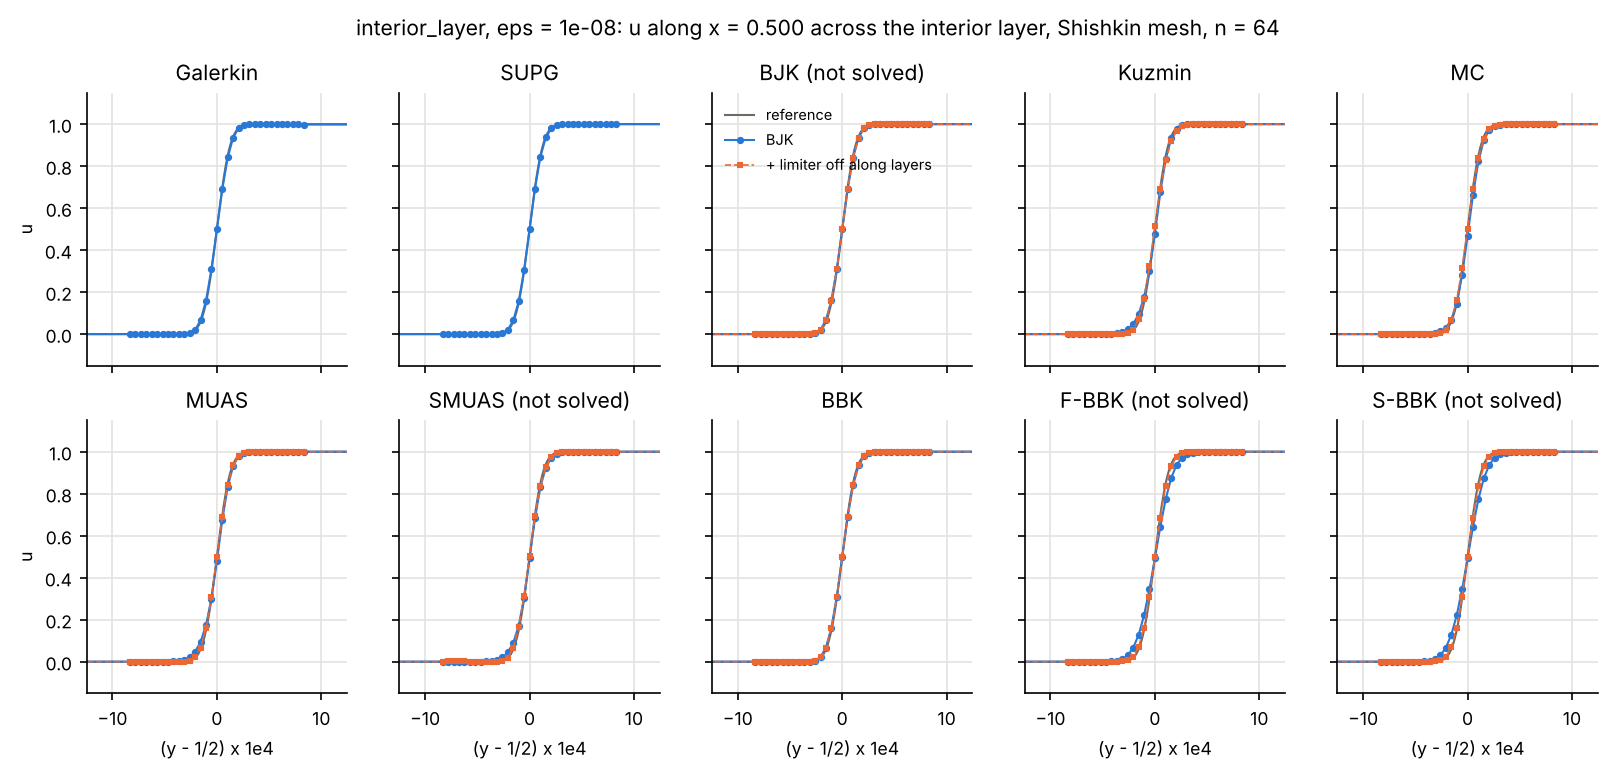
\includegraphics[width=\textwidth]{figures/interior_cut_shishkin_n64.png}
\caption{\texttt{interior\_layer}: $u_h$ along $x\approx\frac12$ across the interior layer (zoom
$|y-\frac12|\le1.5\tau_y$), Shishkin mesh, $n=64$; grey: reference; orange: limiter switched off along the
layers.}\label{fig:interior-cut}
\end{figure}

\begin{figure}[!htbp]
\centering
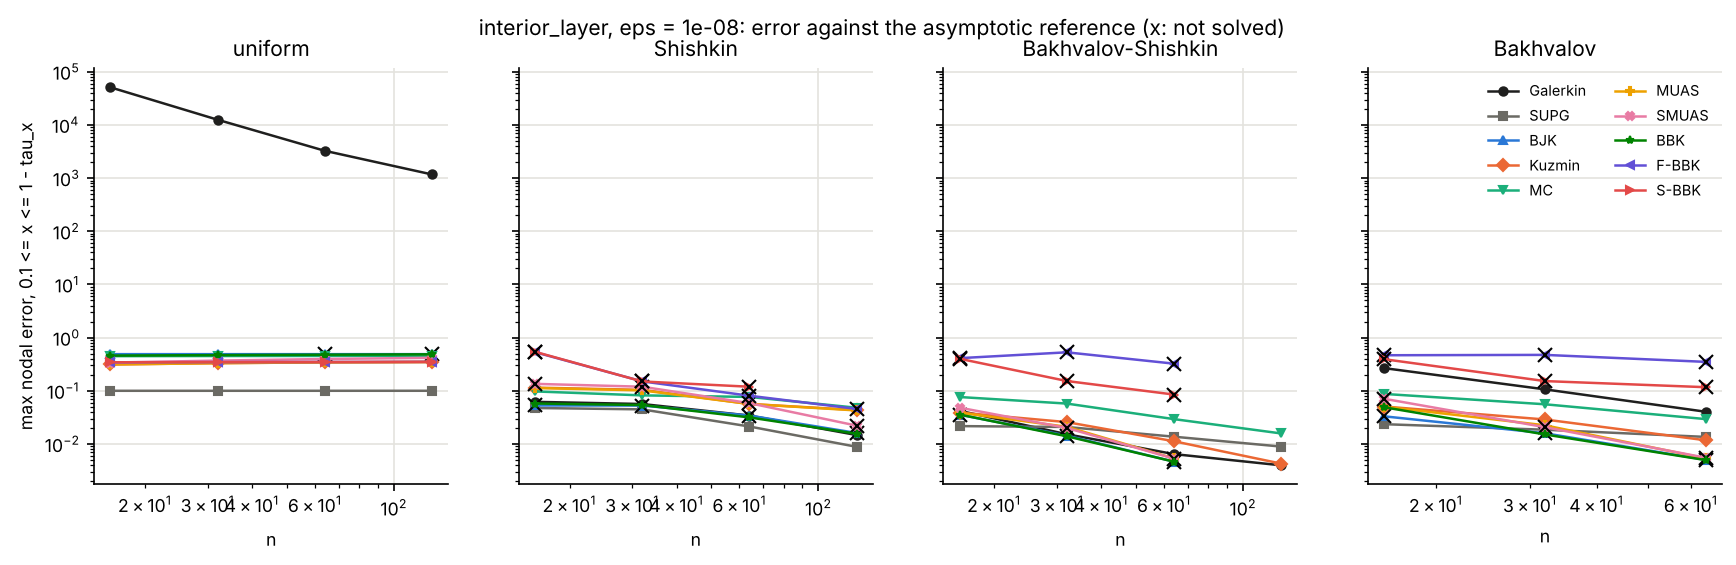
\includegraphics[width=\textwidth]{figures/interior_errors.png}
\caption{\texttt{interior\_layer}: maximal nodal error for $0.1\le x\le1-\tau_x$ against $n$; crosses: nonlinear
problem not solved.}\label{fig:interior-err}
\end{figure}

\paragraph{Results} (Table~\ref{tab:interior}, Figures~\ref{fig:interior-cut}, \ref{fig:interior-err}).
\begin{itemize}[leftmargin=*]
\item \textbf{The algebraic methods are the most accurate here.} On the Bakhvalov--Shishkin and Bakhvalov meshes
  BBK, MUAS and SMUAS have $L^2$ errors of $3.3$--$4.3\cdot10^{-5}$ at $n=64$, 30 times smaller than Galerkin
  ($1.2\cdot10^{-3}$) and 5 times smaller than SUPG ($2\cdot10^{-4}$), and they keep $u_h\le1$; Galerkin and SUPG
  overshoot by 0.4--1.8\,\%. The solution is monotone across the layer, so the limiters have no genuine extremum
  to clip.
\item \textbf{The Bakhvalov-type meshes are much better than the Shishkin mesh} for this layer: about a factor 10 in
  the errors of all methods; the abrupt transition of the Shishkin mesh at the edge of the layer region costs
  accuracy.
\item \textbf{The switch along the layers} lowers the maximal error of some methods (Kuzmin on the
  Bakhvalov--Shishkin mesh $1.1\cdot10^{-2}\to4.4\cdot10^{-3}$) but brings back overshoots of 0.3--0.6\,\%.
\item On the uniform mesh the layer is not resolved: Galerkin is useless, and the algebraic methods smear it over a
  width about 100 times the reference width.
\end{itemize}

%=====================================================================================================
\section{Transport of a profile along circles}\label{sec:rotating}
%=====================================================================================================

\paragraph{Problem \texttt{rotating\_profile}.} The steady example of arXiv:2204.07480, Section~7, as it was given to
us: $\eps=10^{-5}$, $\bb=(-y,x)$, $c=f=0$ on $(0,1)^2$; at the inlet $y=0$
\[
  u(x,0)=\begin{cases}\frac{x-0.375}{\xi}+1, & x\in[0.375-\xi,0.375),\\
  -0.75\,\frac{x-0.5}{0.125}+0.25, & x\in[0.375,0.5),\\
  0.25\,\frac{x-0.625}{0.125}+0.5, & x\in[0.5,0.625),\\
  -0.5\,\frac{x-0.625}{\xi}+0.5, & x\in[0.625,0.625+\xi),\\
  32(x-0.75)(1-x), & x\in[0.75,1],\\ 0 & \text{else},\end{cases}\qquad\xi=10^{-3},
\]
$u=0$ at $x=1$ and homogeneous Neumann conditions on $x=0$ and $y=1$ (the outlets). The profile is transported along
the circles $r=\sqrt{x^2+y^2}=$ const: steep interior layers along the arcs $r\approx0.375$ (a ramp $0\to1$) and
$r\approx0.625$ (a drop $0.5\to0$), weak layers (kinks) along $r=0.5$ and $0.75$, and a hump; $0\le u\le1$. The
quantities of interest of that paper could not be used (the paper was not accessible from our environment); the
quantities below are our own.

\paragraph{Reference.} In polar coordinates $\bb\cdot\nabla u=u_\theta$; without the term $\eps u_{\theta\theta}/r^2$,
which is small against $\eps u_{rr}$ in the thin layers, the problem is the radial heat equation
$u_\theta=\eps(u_{rr}+u_r/r)$ in the ``time'' $\theta\in[0,\pi/2]$ with the inflow profile as initial value. It is
solved with $4\cdot10^4$ radial cells and $4000$ Crank--Nicolson steps; halving both changes it by $3\cdot10^{-5}$.

\paragraph{Meshes} (all with about $n\times n$ cells; Figure~\ref{fig:rot-sol}, first column).
\begin{itemize}[leftmargin=*]
\item \emph{uniform};
\item \emph{polar}: rings $r=$ const, uniform in $r$ up to $0.9$ and then blended to the square, $n$ uniform angles
  (\texttt{polar\_square\_mesh}); aligned with the layers;
\item \emph{polar, layer-adapted}: the polar mesh with Shishkin-type refinement across $r=0.375,0.625$ ($n/4$ rings
  each) and $0.5,0.75$ ($n/10$ each), half-width $\tau=2\sqrt\eps\ln n$ (\texttt{graded\_points}); anisotropic and
  aligned (median aspect ratio about 3);
\item \emph{tensor, layer-refined}: a tensor mesh refined in $x$ and in $y$ at the same four values; anisotropic,
  but aligned with the arcs only near the inlet and the outlet.
\end{itemize}
Variants of the algebraic methods: \emph{+ off}, the limiter switched off along the layers (\texttt{afc\_layer\_off}
with aspect threshold 3, since the polar layer cells are only moderately stretched), and $\mu=2$, the relaxed limiter
$R_i=\min\{1,\mu Q_i/P_i\}$ (\texttt{afc\_q\_relax}; for Kuzmin the form (27) of Knobloch), which limits less but no
longer guarantees the DMP. For the Neumann vertices BJK uses the convex-hull rule for $\gamma_i$ and SMUAS no
reflected values. Results for $n=32,64$ (the runs at $n=128$ were stopped).

% generated by galerkit examples/convection_diffusion/2d/anisotropic_afc/make_report.py; do not edit
\begin{table}[!htbp]
\centering\scriptsize\setlength{\tabcolsep}{3pt}
\caption{\texttt{rotating\_profile}, $\varepsilon=10^{-5}$, $n=64$: $L^2$ error ($r\le1$) against the radial reference and undershoot $-\min u_h$ (the overshoots are below $2\cdot10^{-5}$ except Galerkin/SUPG on the uniform and tensor meshes, $0.02$--$0.3$); + off: limiter switched off along the layers (aspect threshold 3); $\mu=2$: relaxed limiter; $^*$: nonlinear problem not solved.}\label{tab:rotating}
\resizebox{\textwidth}{!}{\begin{tabular}{l rr rr rr rr}
\toprule
 & \multicolumn{2}{c}{uniform} & \multicolumn{2}{c}{polar} & \multicolumn{2}{c}{polar, layer-adapted} & \multicolumn{2}{c}{tensor, layer-refined}\\
method & $L^2$ & under. & $L^2$ & under. & $L^2$ & under. & $L^2$ & under.\\
\midrule
Galerkin & $5.6\mathrm{e}{-2}$ & $1.6\mathrm{e}{-1}$ & $2.1\mathrm{e}{-2}$ & $4.6\mathrm{e}{-2}$ & $1.2\mathrm{e}{-2}$ & $4.5\mathrm{e}{-2}$ & $7.2\mathrm{e}{-2}$ & $4.5\mathrm{e}{-1}$ \\
SUPG & $5.3\mathrm{e}{-2}$ & $7.9\mathrm{e}{-2}$ & $2.2\mathrm{e}{-2}$ & $2.2\mathrm{e}{-2}$ & $1.3\mathrm{e}{-2}$ & $2.4\mathrm{e}{-2}$ & $6.3\mathrm{e}{-2}$ & $1.1\mathrm{e}{-1}$ \\
BJK & $5.9\mathrm{e}{-2}$ & 0 & $4.1\mathrm{e}{-2}$$^*$ & $3.9\mathrm{e}{-6}$ & $4.2\mathrm{e}{-2}$$^*$ & 0 & $6.5\mathrm{e}{-2}$$^*$ & 0 \\
BJK + off & -- & -- & $4.0\mathrm{e}{-2}$$^*$ & $3.2\mathrm{e}{-2}$ & $1.7\mathrm{e}{-2}$$^*$ & $3.4\mathrm{e}{-2}$ & $6.2\mathrm{e}{-2}$$^*$ & $3.3\mathrm{e}{-1}$ \\
BJK, $\mu=2$ & $5.4\mathrm{e}{-2}$$^*$ & 0 & $9.1\mathrm{e}{-2}$$^*$ & $3.7\mathrm{e}{-2}$ & $3.1\mathrm{e}{-2}$$^*$ & $1.8\mathrm{e}{-8}$ & $6.2\mathrm{e}{-2}$$^*$ & $2.4\mathrm{e}{-6}$ \\
Kuzmin & $6.8\mathrm{e}{-2}$ & 0 & $7.1\mathrm{e}{-2}$ & 0 & $6.8\mathrm{e}{-2}$ & 0 & $1.0\mathrm{e}{-1}$ & 0 \\
Kuzmin + off & -- & -- & $7.0\mathrm{e}{-2}$ & $6.8\mathrm{e}{-3}$ & $5.1\mathrm{e}{-2}$ & $7.5\mathrm{e}{-3}$ & $8.4\mathrm{e}{-2}$ & $3.0\mathrm{e}{-1}$ \\
Kuzmin, $\mu=2$ & $6.1\mathrm{e}{-2}$ & 0 & $5.4\mathrm{e}{-2}$$^*$ & $3.0\mathrm{e}{-6}$ & $5.7\mathrm{e}{-2}$ & 0 & $8.3\mathrm{e}{-2}$ & 0 \\
MC & $6.6\mathrm{e}{-2}$ & 0 & $6.8\mathrm{e}{-2}$ & 0 & $6.3\mathrm{e}{-2}$ & 0 & $9.3\mathrm{e}{-2}$ & 0 \\
MC + off & -- & -- & $6.7\mathrm{e}{-2}$ & $3.2\mathrm{e}{-3}$ & $2.9\mathrm{e}{-2}$ & $4.3\mathrm{e}{-3}$ & $7.7\mathrm{e}{-2}$ & $3.5\mathrm{e}{-1}$ \\
MUAS & $6.8\mathrm{e}{-2}$ & 0 & $7.1\mathrm{e}{-2}$ & 0 & $6.8\mathrm{e}{-2}$ & 0 & $1.0\mathrm{e}{-1}$ & 0 \\
MUAS + off & -- & -- & $6.9\mathrm{e}{-2}$ & $3.5\mathrm{e}{-3}$ & $2.9\mathrm{e}{-2}$ & $2.9\mathrm{e}{-3}$ & $8.2\mathrm{e}{-2}$ & $3.4\mathrm{e}{-1}$ \\
MUAS, $\mu=2$ & $6.1\mathrm{e}{-2}$ & 0 & $5.4\mathrm{e}{-2}$$^*$ & $4.7\mathrm{e}{-6}$ & $5.7\mathrm{e}{-2}$ & 0 & $8.2\mathrm{e}{-2}$ & 0 \\
SMUAS & $8.1\mathrm{e}{-2}$ & 0 & $8.8\mathrm{e}{-2}$ & 0 & $7.3\mathrm{e}{-2}$ & 0 & $1.0\mathrm{e}{-1}$ & 0 \\
SMUAS + off & -- & -- & $8.6\mathrm{e}{-2}$ & $7.0\mathrm{e}{-3}$ & $4.3\mathrm{e}{-2}$ & $7.8\mathrm{e}{-3}$ & $8.8\mathrm{e}{-2}$ & $3.0\mathrm{e}{-1}$ \\
SMUAS, $\mu=2$ & $6.7\mathrm{e}{-2}$ & 0 & $6.7\mathrm{e}{-2}$ & 0 & $6.2\mathrm{e}{-2}$ & 0 & $8.3\mathrm{e}{-2}$ & 0 \\
BBK & $5.9\mathrm{e}{-2}$ & 0 & $4.6\mathrm{e}{-2}$$^*$ & $4.8\mathrm{e}{-6}$ & $5.1\mathrm{e}{-2}$ & 0 & $7.3\mathrm{e}{-2}$ & 0 \\
BBK + off & -- & -- & $4.5\mathrm{e}{-2}$ & $2.6\mathrm{e}{-2}$ & $1.9\mathrm{e}{-2}$ & $2.6\mathrm{e}{-2}$ & $6.7\mathrm{e}{-2}$ & $3.0\mathrm{e}{-1}$ \\
F-BBK & $8.1\mathrm{e}{-2}$$^*$ & $8.9\mathrm{e}{-6}$ & $1.3\mathrm{e}{-1}$$^*$ & $3.3\mathrm{e}{-4}$ & $9.4\mathrm{e}{-2}$$^*$ & 0 & $1.2\mathrm{e}{-1}$$^*$ & $3.5\mathrm{e}{-3}$ \\
F-BBK + off & -- & -- & $7.3\mathrm{e}{-2}$$^*$ & $3.5\mathrm{e}{-3}$ & $4.5\mathrm{e}{-2}$$^*$ & $4.6\mathrm{e}{-3}$ & $1.1\mathrm{e}{-1}$$^*$ & $3.3\mathrm{e}{-2}$ \\
S-BBK & $8.1\mathrm{e}{-2}$$^*$ & $8.9\mathrm{e}{-6}$ & $1.3\mathrm{e}{-1}$$^*$ & $2.6\mathrm{e}{-5}$ & $6.8\mathrm{e}{-2}$ & 0 & $1.1\mathrm{e}{-1}$ & $2.7\mathrm{e}{-4}$ \\
S-BBK + off & -- & -- & $7.4\mathrm{e}{-2}$$^*$ & $3.2\mathrm{e}{-3}$ & $5.4\mathrm{e}{-2}$$^*$ & $4.5\mathrm{e}{-3}$ & $9.8\mathrm{e}{-2}$$^*$ & $3.8\mathrm{e}{-2}$ \\
\bottomrule
\end{tabular}}
\end{table}


\begin{figure}[!htbp]
\centering
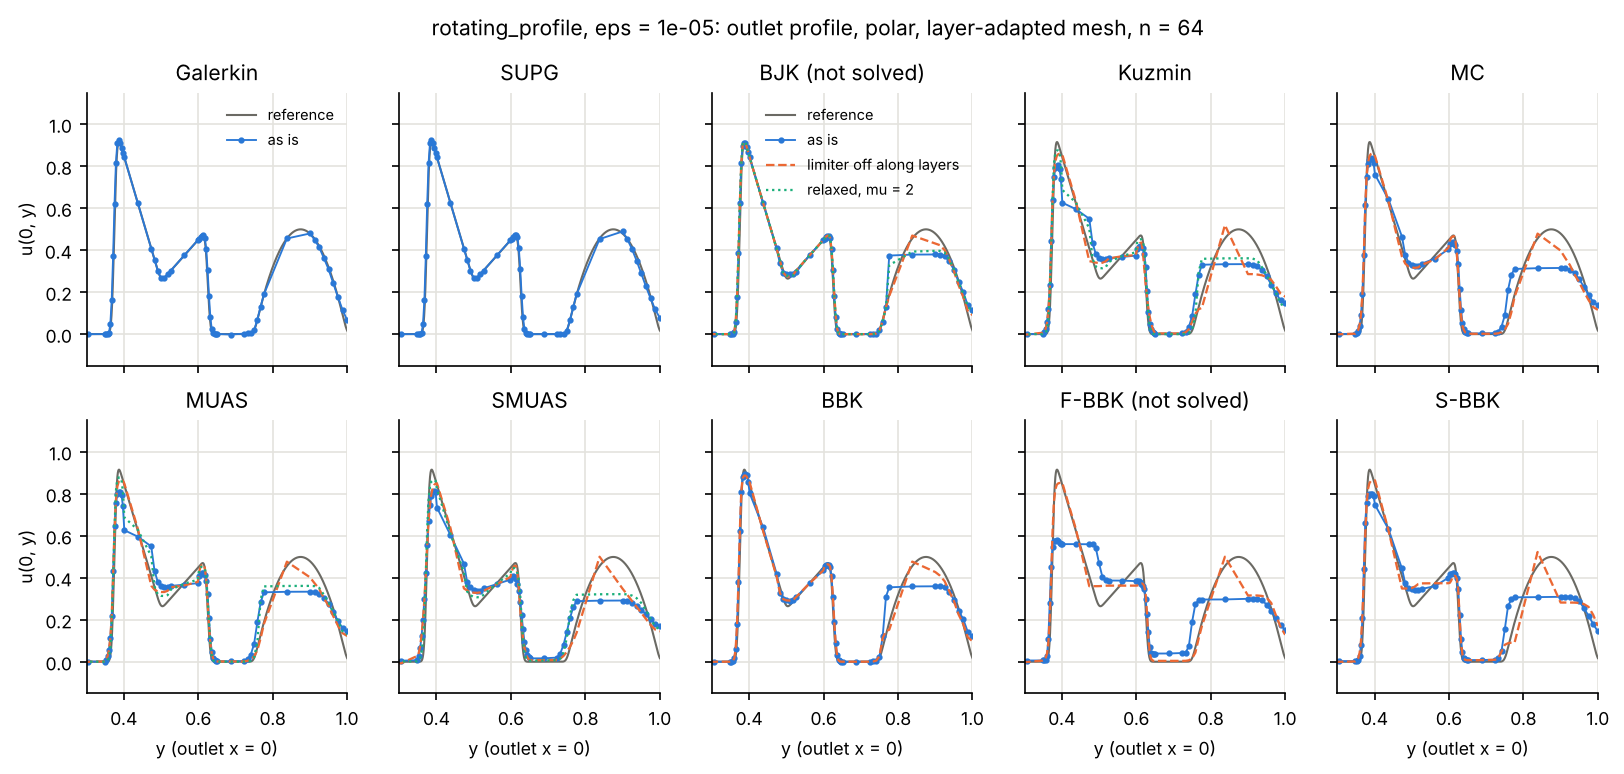
\includegraphics[width=\textwidth]{figures/rotating_outlet_polar_layer_n64.png}
\caption{\texttt{rotating\_profile}: outlet profile $u_h(0,y)$ on the layer-adapted polar mesh, $n=64$; grey:
reference; blue: the method; orange: limiter off along the layers; green: $\mu=2$.}\label{fig:rot-outlet}
\end{figure}

\begin{figure}[!htbp]
\centering
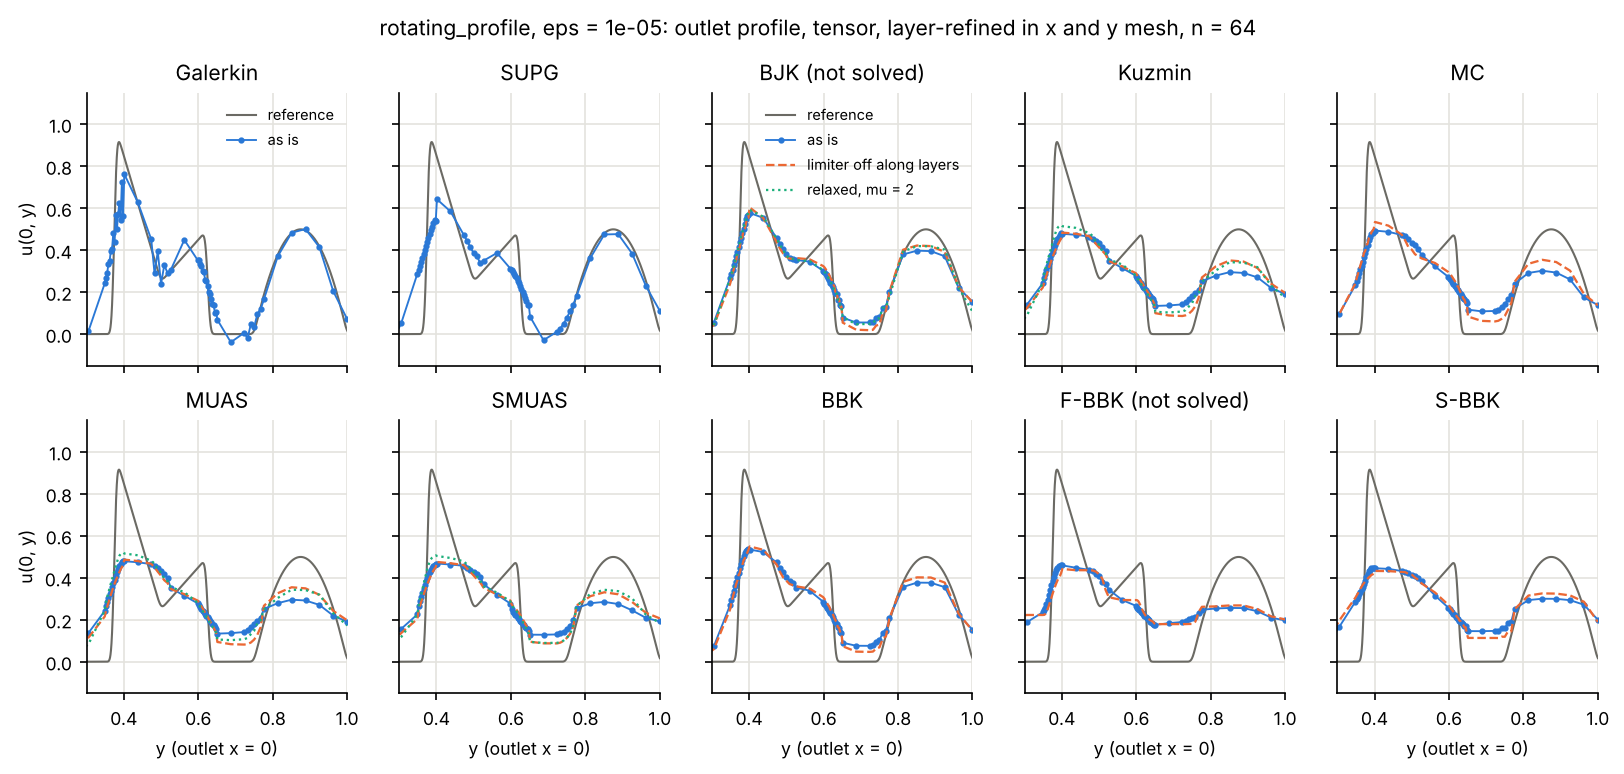
\includegraphics[width=\textwidth]{figures/rotating_outlet_tensor_layer_n64.png}
\caption{\texttt{rotating\_profile}: outlet profile on the tensor mesh refined in $x$ and $y$, $n=64$.}
\label{fig:rot-outlet-tensor}
\end{figure}

\begin{figure}[!htbp]
\centering
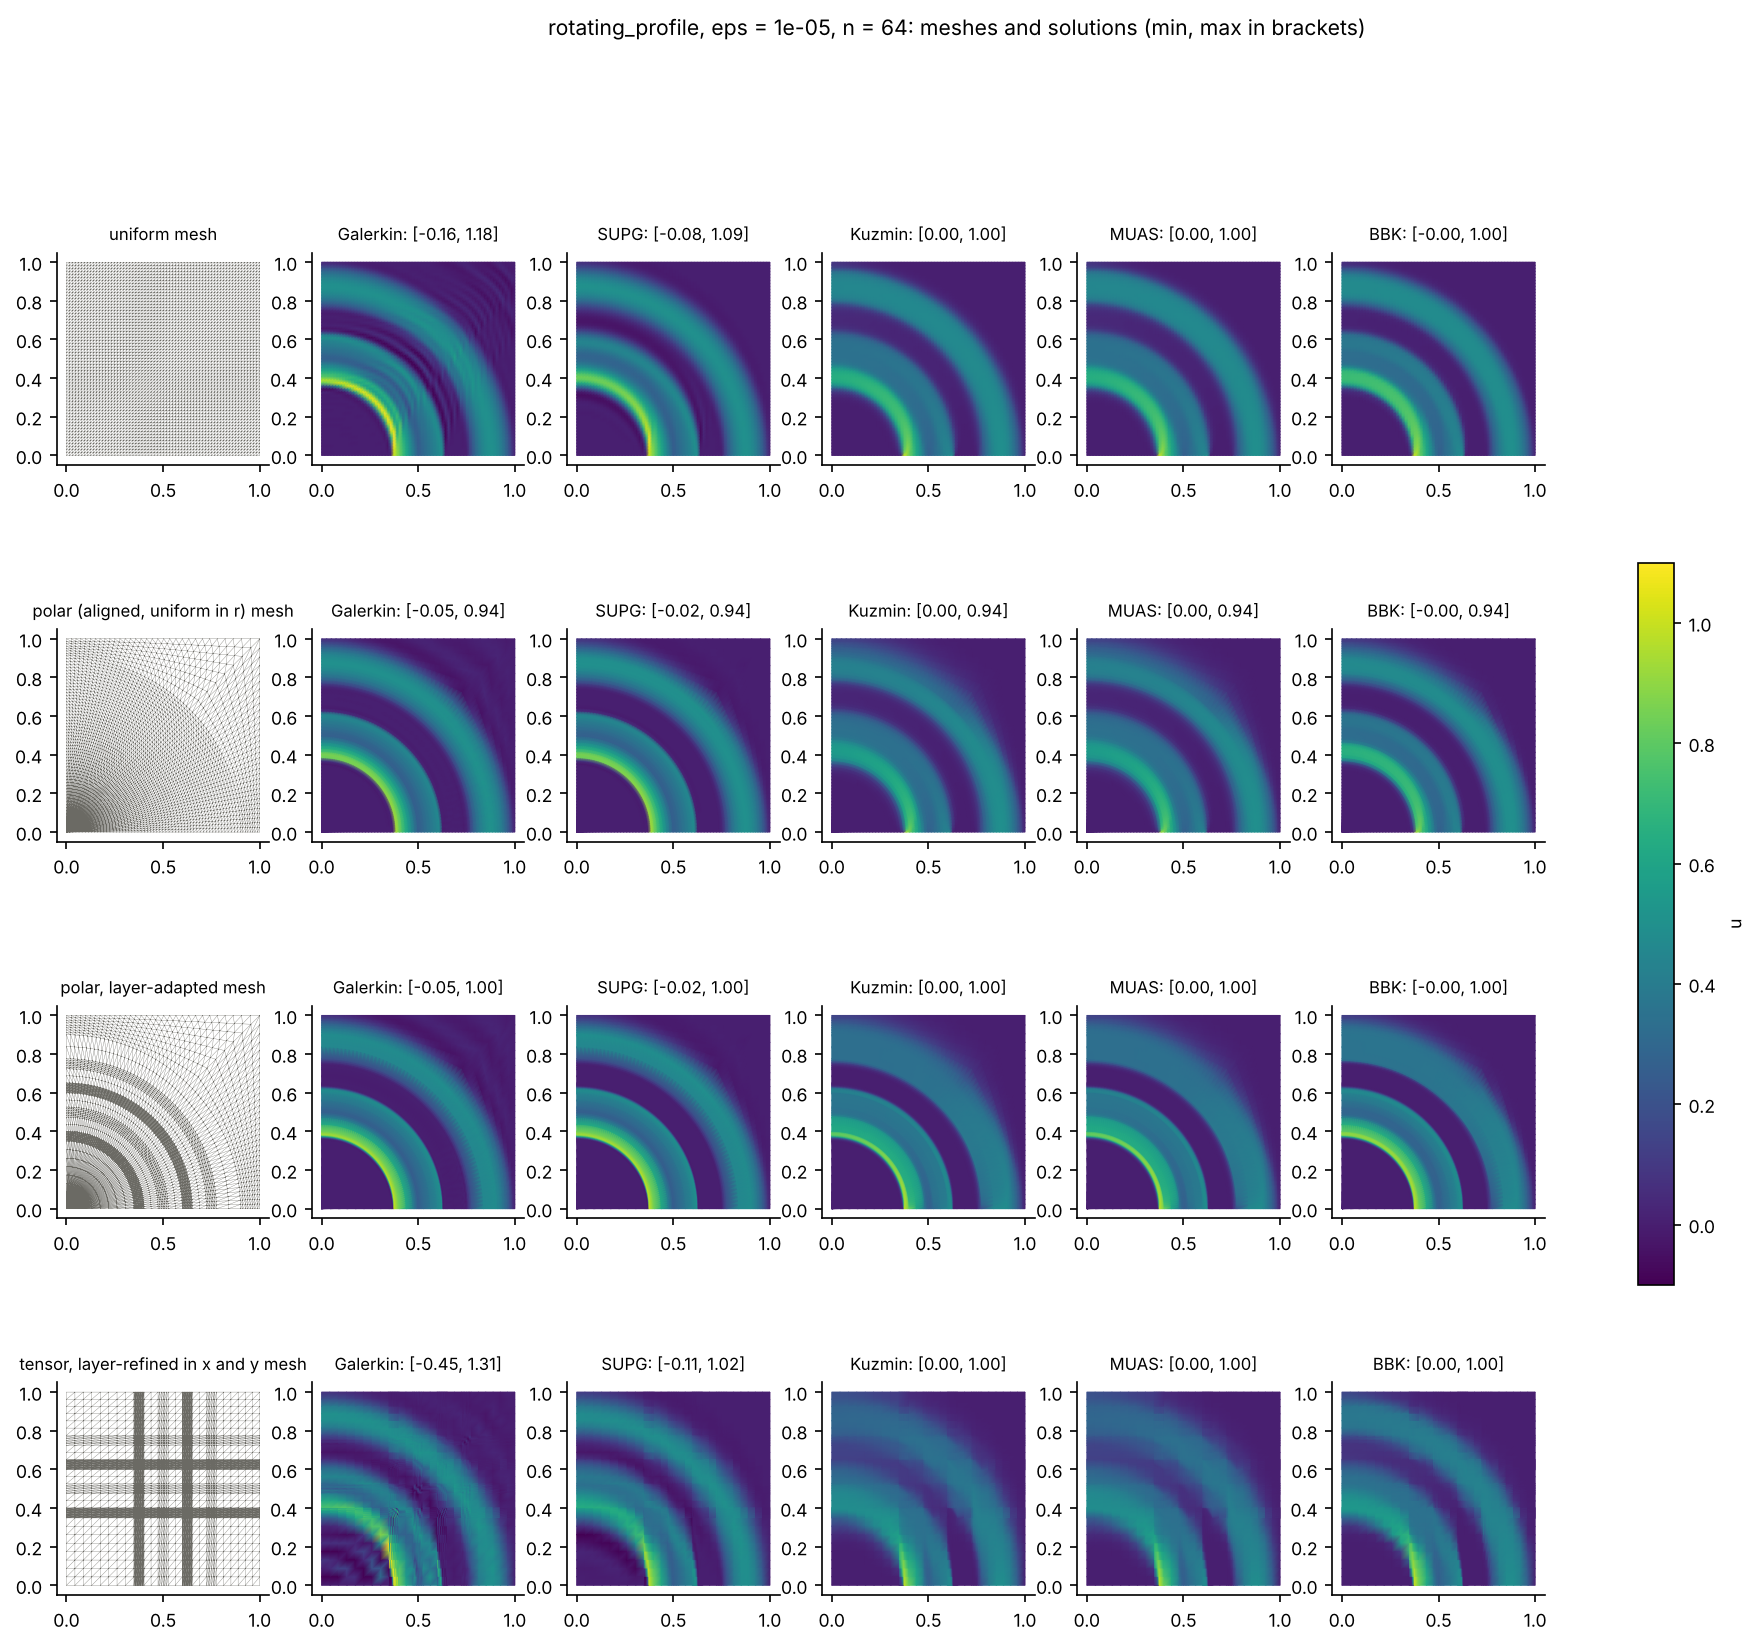
\includegraphics[width=\textwidth]{figures/rotating_solutions_n64.png}
\caption{\texttt{rotating\_profile}, $n=64$: the four meshes and the solutions of Galerkin, SUPG, Kuzmin, MUAS and
BBK ($\min u_h$, $\max u_h$ in brackets).}\label{fig:rot-sol}
\end{figure}

\paragraph{Results} (Table~\ref{tab:rotating}, Figures~\ref{fig:rot-outlet}--\ref{fig:rot-sol}).
\begin{itemize}[leftmargin=*]
\item \textbf{The mesh matters most.} The layer-adapted polar mesh is the best for every method; the tensor mesh
  refined in $x$ and $y$ is the worst for every method, worse than the uniform mesh, since in the middle of the domain
  it is fine in directions that do not cross the arcs.
\item \textbf{On the aligned mesh Galerkin and SUPG are the most accurate} ($L^2$ error $1.2$--$1.3\cdot10^{-2}$ at
  $n=64$) but undershoot by 2--5\,\%. The algebraic methods keep $0\le u_h\le1$ and are 3.5--6 times less accurate:
  their limiters cannot distinguish the genuine extrema of the profile (the peak behind $r=0.375$, the minimum at the
  kink $r=0.5$, the top of the hump) from oscillations, switch to the low-order scheme there along the whole
  streamline, and clip them (Figure~\ref{fig:rot-outlet}); the diagonal edges of the polar cells add crosswind
  diffusion.
\item \textbf{The switch along the layers closes most of the gap} on the aligned mesh: BJK $1.7\cdot10^{-2}$, BBK
  $1.9\cdot10^{-2}$, MC and MUAS $6.8\to2.9\cdot10^{-2}$; it recovers the peak and most of the hump, at the price of
  undershoots of 0.3--0.4\,\% (MC, MUAS) and 3\,\% (BJK, BBK). On the misaligned tensor mesh it is harmful
  (undershoots of 30\,\%).
\item \textbf{The relaxed limiter $\mu=2$ helps little} (Kuzmin, MUAS $6.8\to5.7\cdot10^{-2}$) and keeps the bounds.
\item Accurate and almost bound-preserving: MC or MUAS with the switch on the layer-adapted polar mesh; most accurate
  with small undershoots: SUPG on that mesh. BJK and F-BBK are not solved in several runs.
\end{itemize}

%=====================================================================================================
\section{Conclusions and next steps}
%=====================================================================================================

\begin{enumerate}[leftmargin=*]
\item On layer-adapted meshes all algebraic stabilizations resolve the layers, but they reduce the accuracy compared
  with the Galerkin method, which is stable there; the error concentrates at the transition corner. Switching the
  stabilization off on edges with mesh P\'eclet number $\le1$ (\texttt{afc\_resolved\_off}) does not help
  (Section~\ref{sec:roff}): the methods add no diffusion on those edges anyway, and the harmful diffusion acts on the
  long, unresolved edges along the layers.
\item The nonlinear problems become harder on anisotropic meshes. Kuzmin and MUAS remain the most robust; SMUAS, which
  is the most accurate method on general isotropic meshes, often fails to converge on Shishkin meshes.
\item The DMP conditions of the restricted methods are satisfied on Shishkin meshes split into right triangles and
  violated on crossed splittings, without observed DMP violations; the guaranteed methods need no condition. For
  anisotropic meshes the splitting into right triangles is therefore the safe choice.
\item Switching the limiter off on the long edges along the layers (\texttt{afc\_layer\_off},
  Section~\ref{sec:loff}) reduces the fixed point iterations by factors 3--50 and the error at the transition corner
  by up to a factor 5. Smoother layer-adapted meshes (Bakhvalov--Shishkin, Bakhvalov, Dur\'an--Lombardi;
  Section~\ref{sec:meshes}) change the iterations by at most a factor 2 in either direction; with the switch the mesh
  type hardly matters. Fewest iterations: Shishkin mesh, switch on, Kuzmin or MUAS.
\item Anderson acceleration on top of the switch (Section~\ref{sec:aa}) reduces the iterations further, by a factor 3--4
  for \texttt{boundary\_layers} (Kuzmin and MUAS: 35--37 on the Shishkin mesh) and lets SMUAS converge there; with
  the non-monotone safeguard (\texttt{fp\_anderson\_safe}) F-BBK and S-BBK converge too. It does not help for the
  parabolic layers. Fewest iterations overall: Shishkin mesh, \texttt{afc\_layer\_off}, \texttt{fp\_anderson\_safe},
  Kuzmin or MUAS.
\item For the parabolic layers, Newton's method with regularized ($C^1$) limiters, continuation in the regularization
  and a final Newton step on the original scheme (Section~\ref{sec:nreg}) solves BBK in all 12 runs (25--65 steps; fixed
  point 1, Anderson 5), and Kuzmin and MUAS in 26--75 steps; BJK, SMUAS, F-BBK and S-BBK remain unsolved.
\item Interior layers (Sections~\ref{sec:interior}, \ref{sec:rotating}): for a straight interior layer with a monotone
  profile across it the algebraic methods on Bakhvalov-type meshes are the most accurate (BBK, MUAS, SMUAS: $L^2$
  errors 30 times below Galerkin, no overshoots). For a profile with genuine extrema transported along circles the
  layer-aligned (polar, layer-adapted) mesh is essential, Galerkin and SUPG are the most accurate but violate the
  bounds, and the algebraic methods clip the extrema; switching the limiter off along the layers recovers most of the
  accuracy with undershoots below 0.4\,\% (MC, MUAS).
\item Open: the quantities of interest of arXiv:2204.07480 for the rotating profile, limiters that do not clip smooth
  extrema, anisotropic meshes not aligned with the axes, 3D, the solver failures of SMUAS on
  \texttt{boundary\_layers}, and the role of $\sigma$ in the transition point.
\end{enumerate}

\paragraph{Reproducibility.} galerkit branch \texttt{feature/anisotropic-afc}, folder
\begin{center}\texttt{examples/convection\_diffusion/2d/anisotropic\_afc}:\end{center}
\texttt{run\_aniso.py} (the runs), \texttt{interior\_layer.py} and \texttt{rotating\_profile.py} (the examples of
Sections~\ref{sec:interior}, \ref{sec:rotating}), \texttt{make\_report.py} (these tables and figures) and
\texttt{results.json}. The latter holds the 3547 runs of \texttt{run\_aniso.py}:
\begin{itemize}[leftmargin=*,nosep]
\item 638 on uniform and Shishkin meshes, 63 with \texttt{afc\_resolved\_off}, 507 with \texttt{afc\_layer\_off},
  480 on the graded meshes;
\item 991 with Anderson acceleration;
\item 868 with Newton and regularized limiters (784 with the exact Jacobian on all problems and meshes, 84 with the
  finite difference one).
\end{itemize}
F-BBK and S-BBK on the crossed Shishkin mesh of \texttt{parabolic\_layers} at $n=128$ were stopped after more than an
hour and are missing; so are the runs at $n=128$ of the two examples of Sections~\ref{sec:interior} and
\ref{sec:rotating}.

\end{document}
